\documentclass[12pt,]{article}
\usepackage{lmodern}
\usepackage{amssymb,amsmath}
\usepackage{ifxetex,ifluatex}
\usepackage{fixltx2e} % provides \textsubscript
\ifnum 0\ifxetex 1\fi\ifluatex 1\fi=0 % if pdftex
  \usepackage[T1]{fontenc}
  \usepackage[utf8]{inputenc}
\else % if luatex or xelatex
  \ifxetex
    \usepackage{mathspec}
    \usepackage{xltxtra,xunicode}
  \else
    \usepackage{fontspec}
  \fi
  \defaultfontfeatures{Mapping=tex-text,Scale=MatchLowercase}
  \newcommand{\euro}{€}
\fi
% use upquote if available, for straight quotes in verbatim environments
\IfFileExists{upquote.sty}{\usepackage{upquote}}{}
% use microtype if available
\IfFileExists{microtype.sty}{%
\usepackage{microtype}
\UseMicrotypeSet[protrusion]{basicmath} % disable protrusion for tt fonts
}{}
\usepackage[margin=1in]{geometry}
\ifxetex
  \usepackage[setpagesize=false, % page size defined by xetex
              unicode=false, % unicode breaks when used with xetex
              xetex]{hyperref}
\else
  \usepackage[unicode=true]{hyperref}
\fi
\hypersetup{breaklinks=true,
            bookmarks=true,
            pdfauthor={},
            pdftitle={Is the Tea Party Libertarian, Authoritarian, or Something Else?},
            colorlinks=true,
            citecolor=black,
            urlcolor=red,
            linkcolor=black,
            pdfborder={0 0 0}}
\urlstyle{same}  % don't use monospace font for urls
\usepackage{graphicx,grffile}
\makeatletter
\def\maxwidth{\ifdim\Gin@nat@width>\linewidth\linewidth\else\Gin@nat@width\fi}
\def\maxheight{\ifdim\Gin@nat@height>\textheight\textheight\else\Gin@nat@height\fi}
\makeatother
% Scale images if necessary, so that they will not overflow the page
% margins by default, and it is still possible to overwrite the defaults
% using explicit options in \includegraphics[width, height, ...]{}
\setkeys{Gin}{width=\maxwidth,height=\maxheight,keepaspectratio}
\setlength{\parindent}{0pt}
\setlength{\parskip}{6pt plus 2pt minus 1pt}
\setlength{\emergencystretch}{3em}  % prevent overfull lines
\providecommand{\tightlist}{%
  \setlength{\itemsep}{0pt}\setlength{\parskip}{0pt}}
\setcounter{secnumdepth}{0}

%%% Use protect on footnotes to avoid problems with footnotes in titles
\let\rmarkdownfootnote\footnote%
\def\footnote{\protect\rmarkdownfootnote}

%%% Change title format to be more compact
\usepackage{titling}

% Create subtitle command for use in maketitle
\newcommand{\subtitle}[1]{
  \posttitle{
    \begin{center}\large#1\end{center}
    }
}

\setlength{\droptitle}{-2em}
  \title{Is the Tea Party Libertarian, Authoritarian, or Something Else?
\vspace{1.25em}}
  \pretitle{\vspace{\droptitle}\centering\huge}
  \posttitle{\par}
  \author{}
  \preauthor{}\postauthor{}
  \date{}
  \predate{}\postdate{}

\usepackage{setspace}

% Redefines (sub)paragraphs to behave more like sections
\ifx\paragraph\undefined\else
\let\oldparagraph\paragraph
\renewcommand{\paragraph}[1]{\oldparagraph{#1}\mbox{}}
\fi
\ifx\subparagraph\undefined\else
\let\oldsubparagraph\subparagraph
\renewcommand{\subparagraph}[1]{\oldsubparagraph{#1}\mbox{}}
\fi

\begin{document}
\maketitle

\doublespacing

Scholars have been fascinated by the Tea Party since it first emerged on
the American political scene in the spring of 2009. While some have
dismissed it as simply a repackaging of conventional American
conservative populism, many have been struck by how effective it has
been in remobilizing the Republican Party base in the wake of the
Democratic electoral landslide of 2008. Most of the scholarship has
focused upon the demographic make up of its members (Courser 2012; Disch
2011; Maxwell and Parent 2012; Williamson, Skocpol, and Coggin 2011),
how it combines elements of elite and grassroots political mobilization
in new and innovative ways (Bailey, Mummolo, and Noel 2012; Karpowitz et
al. 2011), how it is a racialized response to the election of the first
African American President (Abramowitz 2012; Bailey, Mummolo, and Noel
2012; Disch 2011; Lowndes 2012; Skocpol and Williamson 2012) and how it
might connect with more militarized elements of the American far right
(Parker and Barreto 2013; Skocpol and Williamson 2012). Less attention
has been paid to the question of whether or not a specific ideology
might be driving support for the Tea Party. When ideology is explicitly
addressed, authors tend to note a peculiar contradiction in core beliefs
of Tea Party supporters: the Tea Party seems to embody an odd fusion of
libertarianism and social conservatism (Arceneaux and Nicholson 2012;
Berlet 2012; P. Montgomery 2012; Parker and Barreto 2013; Williamson,
Skocpol, and Coggin 2011; Wilson and Burack 2012). While we agree with
previous scholars who observe that the Tea Party does not have one
unifying ideology, we believe that political scientists have so far
underestimated or incompletely specified the unique ideological drivers
of Tea Party support.

The central claim of this article is that a crucial ideological factor
explaining support for the Tea Party is what Friedrich Nietzsche called
``misarchism'' in reference to the political philosophy of Herbert
Spencer. As we explain in detail below, distinct from both
libertarianism and social conservatism, misarchism refers to an aversion
to \emph{government} combined with support for the \emph{state} and
traditional morality. Consistent with the hypothesis of a misarchist
dimensionality in American attitudes, factor analysis on nine variables
from the 2012 American National Election Time-Series Study (ANES)
reveals that attitudes toward state power are positively intercorrelated
with attitudes toward traditional morality. Though neither are strongly
intercorrelated with attitudes toward government, the factor underlying
support for the state and traditional morality (which we call ``moral
statism'') is strongly and negatively correlated with the factor
underlying support for government. These results are consistent with the
Nietzschean diagnosis of misarchism as an ideological structure which
combines support for the state and moral traditionalism which is
distinct from, and opposed to, attitudes toward government. Consistent
with the argument that misarchism is a crucial ideological driver of
support for the Tea Party, regression analyses reveal that the
interaction of moral statism with governmentalism (our
operationalization of misarchism) has, of all the independent variables
considered, one of the strongest and most robust partial correlations
with support for the Tea Party. Our findings have important implications
for our understanding of right-wing ideology in the United States and
they help to resolve the puzzle of the Tea Party's still poorly
understood and contradictory ideological components.

The article proceeds in five sections. The first section elaborates the
puzzle of the Tea Party's ideological composition. The second section
details the theory that misarchism is a component of the Tea Party's
ideological composition. The third section explains our research
strategy, including a discussion of our data and modeling approach. A
fourth section presents the analysis with a discussion of findings and a
fifth section concludes.

\subsection{The Tea Party: Libertarians, Social Conservatives, Both, or
Something
Else?}\label{the-tea-party-libertarians-social-conservatives-both-or-something-else}

There are currently two dominant accounts of Tea Party ideology in the
academic literature. The first approach argues that Tea Party support is
driven largely by far right-wing support within the Republican Party
(Burack and Snyder-Hall 2012; Parker and Barreto 2013; Skocpol and
Williamson 2012). The second approach downplays the role of ideology by
contending that the Tea Party does not represent the ideology of members
but is rather a decentralized group of diverse viewpoints exploited by
party elites (Bailey, Mummolo, and Noel 2012; Karpowitz et al. 2011; Lo
2012; Williamson, Skocpol, and Coggin 2011). The first approach uses the
standard linear conceptualization of ideology as ranging from left to
right along a single dimension (Knight 2006, 619), whereas the second
approach denies that ideology has much of a role in explaining Tea Party
support. Contra the first account of the Tea Party, we think that the
specific ideology of ``misarchism'' can explain some important
differences between Tea Party members and other conservatives that is
not easily captured in the left-right conceptualization of ideology.
Contra the second account of the Tea Party, our argument is that
ideology can explain an important aspect of Tea Party support.

One prominent example of explaining Tea Party supporters as consisting
largely of the ``far right'' of the American political spectrum is the
detailed analysis of the Tea Party by Christopher S. Parker and Matt A.
Barreto. They argue that the Tea Party is the latest manifestation of
``reactionary conservatism'' (Parker and Barreto 2013; Robin 2013). They
describe reactionary conservatives as individuals on the far right of
the political spectrum who participate in a ``paranoid style'' of
politics that sees ``others'' as a threat to the traditional vision of
America. They locate the Tea Party as inheritors of the political
tradition of the John Birch society and the KKK. In their book, they
write: ``We argue that these {[}anti-Obama{]} sentiments are driven by
anxiety associated with the perception that Obama and his confederates
are subversive forces, ones that threaten to steal `their
country.'(Parker and Barreto 2013, 35)'' According to Parker and
Barreto, the election of the USA's first African-American President
mobilized this reactionary strand of conservatism and drove support for
the Tea Party. While there are other examples, the Parker and Barreto
version of Tea Party ideology is emblematic because it considers
ideology in a traditional one-dimensional, left-right spectrum. The
party can be labeled ``reactionary'' because it is further to the right
on the ideological spectrum than ``mainstream'' conservatism (Parker and
Barreto 2013, 48).

The left-right ideological spectrum approach, however, has a difficult
time explaining Tea Party support (Carmines and D'Amico 2014, 214).
Scholars will observe that the movement seems to combine elements of
libertarianism and social conservatism (Wilson and Burack 2012). For
example, Parker and Barreto observe, ``Libertarianism and the anti-gay,
socially conservative impulses create great tension in the Tea Party,
tension that is evident both in campaign websites and Tea Party message
boards'' (Parker and Barreto 2013, 174). Arceneaux and Nicholson also
puzzle over the apparent tensions within Tea Party supporters' beliefs,
writing ``Tea Party supporters are committed to the libertarian themes
emphasized by the movement's leaders, such as limiting the size of
government and lowering taxes. Yet, Tea Party supporters are also very
conservative on abortion and gay marriage, lending support for the
notion that the Tea Party is, at least in terms of political attitudes,
more similar to conservatism (and Republicanism) than libertarianism''
(Arceneaux and Nicholson 2012, 701). Similarly, in their observations of
grassroots Tea Party meetings, Skocpol and Williamson observed that
``Some Tea Partiers are social conservatives focused on moral and
cultural issues ranging from pro-life concerns to worries about the the
impact of recent immigration on the cultural coherence of American life,
while others are much more secular minded libertarians, who stress
individual choice on cultural matters and want the Tea Party as a whole
to give absolute priority to fiscal issues (Skocpol and Williamson 2012,
35).'' All of these different accounts of the Tea Party struggle with
the apparent puzzle of how the Tea Party reconciles its apparently
contradictory commitments to smaller government on the one hand, and
calls for greater government intervention in areas such as morality and
immigration on the other hand.

This synthesis can lead to some apparent contradictions in policy
preferences. First, the Tea Party members (at least in public opinion
polling) seem to favour existing entitlement programs such as Social
Security and Medicare while opposing other programs such as Temporary
Assistance for Needy Families (TANF) and the Affordable Care Act
(Skocpol and Williamson 2012, 54--68). Second, Tea Party members are
quite concerned about government intervention with respect to firearms,
but are strongly in favour of increased intervention in terms of
immigration enforcement and counter-terrorism (Parker and Barreto 2013,
165--72; Skocpol and Williamson 2012, 71--72). Third, while the Tea
Party expresses deep concern about government programs aimed at trying
to alter the behavior of citizens (such as Michelle Obama's anti-obesity
campaign) they also express a general concern that America's moral
collapse is at the root of most contemporary problems (Jones, Cox, and
Navarro-Rivera 2013; McCalmont 2013). We will contend that these
apparent contradictions about Tea Party supporters' policy preferences
make more sense if we view them as expressions of an underlying
misarchist ideology.

\subsection{A Theory of the Tea Party as a Misarchist
Movement}\label{a-theory-of-the-tea-party-as-a-misarchist-movement}

By the term ideology, we do not mean any thing so technical as the
concept deployed by Marx or Althusser.\footnote{In the Marxist
  tradition, the term ideology refers to the way in which existing
  social institutions justify the material conditions of a society and
  defend the interests of the dominant class. See Marx and Engels (Marx
  and Engels 1978) and Althusser (Althusser 1971) for the classic
  statements on ideology from this perspective} By ideology we mean ``a
set of ideas, beliefs, opinions and values that: 1) exhibit a recurring
pattern, 2) are held by significant groups, 3) compete over providing
and controlling plans for public policy, and 4) do so with the aim of
justifying, contesting or changing the social policy and political
arrangements and processes of a political community'' (Freeden 2003,
100). Existing research on the Tea Party has downplayed the ideological
dimension. Parker and Barreto in their research control for ideology as
one possible factor in Tea Party support and find that it is not
statistically significant (Parker and Barreto 2013, 100). Others have
argued that the Tea Party does not have a coherent ideology. Instead it
is more a product of top-down organization via well-funded PACs, wealthy
individuals such as the Koch brothers, and media support through venues
such as Fox News (Lo 2012).

One reason most scholars of the Tea Party neglect the possibility of an
ideological basis for Tea Party support is the influential current of
scholarship which suggests the general public is not characterized by
coherent belief systems (Campbell et al. 1960; Converse 1964; Lewis-Beck
et al. 2008). An overarching argument in this current is that most
citizens' attitudes do not reflect enough information, stability, or
consistency to be considered ideological. Given such findings, how could
a certain ideology help to explain Tea Party support? A burgeoning
research agenda in political psychology suggests that political
attitudes are indeed characterized by substantial, underlying
psychological differences which correlate with ideological
self-placement (Goren 2013; Graham, Haidt, and Nosek 2009; Haidt 2012).
Haidt argues that the difference between liberals, conservatives and
libertarians in the U.S. is that their moral systems are based on
different psychological foundations (Graham, Haidt, and Nosek 2009;
Haidt 2012). In a similar vein, Goren demonstrates that voters do not
vote on liberal-conservative predispositions but rather genuine policy
principles, namely, limited government, traditional morality, and
military strength (Goren 2013). Our argument is that misarchism is a
particular combination of precisely such policy principles, a
combination which represents a unique source of Tea Party support and is
distinct from other ideological currents prominent on the contemporary
American right, namely conventional conservatism and libertarianism.

Nietzsche used the term misarchism as a pejorative term to describe the
biological and political philosophy of Herbert Spencer (Nietzsche 2007,
52). He argued that at the core of Spencer's philosophy was a hatred of
rule (as the term misarchy comes from the Greek roots \emph{misein} for
hatred and \emph{archos} for ruler). Spencer hated the government,
because government polices and regulations limited human freedom.
Spencer believed that the government's practice of conducting the
conduct of individuals would short-circuit the development of his end
goal for society: an individual who would be completely self-reliant and
altruistic. Government policies interfered with the evolutionary
process, and enabled less fit, or unfit individuals to survive.
According to Spencer this was a threat to the overall strength and
health of a society. The government was bad not simply because it
limited negative liberty; it was bad because it threatened the full
development of the species. A society without government would enable
human evolution in both physiological and moral terms. Humans would have
a longer life expectancy, would be stronger, and would develop morally
in a way in which they reconciled altruistic and egoistic impulses.
Eventually a fully morally-evolved person would selfishly pursue ends
that were for the benefit of society as a whole. He labeled this type of
person the ``ideally moral man'' (Spencer 1879, 75).

While many people view Herbert Spencer as a proto-libertarian (Zwolinski
2015), some of his contemporary critics, including Thomas Huxley and
Nietzsche, noticed a peculiar feature of Spencer's political philosophy:
he was opposed to any use of the government to redistribute wealth,
alleviate poverty, to regulate professions such as health care, to fund
and regulate a public education system, or to spend on infrastructure,
yet he was strongly supportive of the state increasing its policing
power to maintain order. In his rejoinder to Spencer, Huxley labeled the
political philosophy alternately ``administrative nihilism'' and
``astynomocracy'' (police government) (Huxley 1871). While Spencer's
vision of a minimalist state appeared to promote human freedom, he had
developed a model that eliminated all the regular administrative
activities that a government engages in and replaced it with a state
that was fully vested in its police powers. In Huxley's mind, one of the
most crucial things a government does is: ``averaging the interests of
the various classes in a community; and a good Parliament is one in
which the parties answering to these respective interests are so
balanced, that their united legislation concedes to each class as much
as consists with the claims of the rest'' (Huxley 1871, 271). Spencer
hated this notion of the government striving to create a public good
through the reconciliation of conflicting interests, because this led to
policies that limited human freedom.

What is crucial in Huxley's critique of Spencer is his observation that
Spencer's political program sought to eliminate the government by
empowering the state. The terms government and state are often used
interchangeably but in order to understand how misarchism works as an
ideology, we need to differentiate these two terms. We follow Max Weber
in defining the state as the ``monopoly on legitimate physical
violence'' (Weber 2004, 33). We follow Michel Foucault in defining
government as the ``\,`the conduct of conduct': a form of activity
aiming to shape, guide or affect the conduct of some person or persons''
(Foucault 1991; Gordon 1991, 2). The state uses its monopoly on violence
to dominate its subjects and punish violations of the law. Conversely
government uses techniques such as education, regulation,
administration, and management to shape human behaviour. While states
have governments, government is not limited to the state. For instance,
both for-profit and non-profit corporations have boards of governors and
business schools teach corporate governance.\footnote{Political theorist
  John Hoffman draws a similar distinction between statism and
  governmentalism, where the state refers to the use of force to tackle
  conflict and the government refers to the use of negotiation and
  arbitration to resolve conflicts of interest (Hoffman 1995)}

Our point is that one can be anti-government while being pro-state. If
this position seems odd it is only because we are seeking to identify an
ideology distinct from more established ideologies about government
authority. Classical libertarians are strongly skeptical of both state
power and government power. Libertarianism as an ideology holds that
individual freedom is the greatest good and favors policies that
maximizes individual freedom in both the economic and social sphere and
seeks to minimize government interference as much as possible (Brennan
2012, 1--3). There are crucial differences in policy preferences between
Tea Party supporters and Libertarians on issues such as NSA
surveillance, the use of drone warfare, aggressive U.S. foreign policy,
and the continuation of the war on drugs. Libertarians tend to oppose
state power in these areas, whereas Tea Party members are more likely to
be supportive of increasing state power in these domains. All these
programs involve increasing the state's use of the instruments of
violence in order to counter perceived threats to the state. Where
libertarians and misarchists agree is on their opposition to
governmentalism; to using government programs and policies to shape the
behaviour of individuals, and to improve the well-being of society.
Traditional conservatives tend to be skeptical of both state power and
governmental power but are more moderate. Conservatism is an ideology
that defends preservation of the status quo and values traditional
social and political structures, preferring incremental social change to
more radical proposals for reform or revolution (Heywood 2007, 65).
Traditional conservatives recognize the need for some statism and some
governmentalism, but are also skeptical of the extremism of both
libertarians and misarchists, who favour the abolition of almost all
government (in both cases) and the minimization of the state (in the
case of libertarians).

One question is whether a possible relationship between misarchism and
support for the Tea Party might only reflect the relationship between
misarchism and Republican Party identification or conservatism more
broadly. In our analysis below, we estimate auxiliary models to see if
the interaction of moral statism and anti-governmentalism also drives
Republican Party identification and/or conservative identification.
While the Republican Party appears to be a ``broad church'' hosting
different strands of conservative ideology, our results support the
argument that misarchism is uniquely associated with Tea Party support.
While there are likely to be conventional conservatives who are
pro-government and morally statist, and libertarians who are
anti-government and anti-moral-statist, it is only our contention that
the Tea Party finds a unique source of support in the combination of
morally statist and anti-government attitudes that we call misarchism.

Based on this reading of Nietzsche, we define misarchism as an
ideological constellation which combines three general attitudes. It
combines attitudes which are 1) anti-government, 2) pro-state, and 3)
moralistic. Anti-government attitudes are those which reflect opposition
to using government policy to improve the condition and behaviour of
individuals and society in general. Misarchists will oppose wealth
redistribution and any programs that aim at assisting individuals in
need. They will also oppose government attempts to regulate individual
behaviour. Pro-state attitudes reflect support for the state using its
monopoly on violence to maintain order and confront perceived threats to
society. Moralistic attitudes are those which see the cultivation of
individual morality rather than government regulation as the best way to
promote a good society.

Conventional taxonomies of ideology tend to line ideologies on a single
dimension from left to right. Thus different strands of conservatism
tend to be categorized as more or less extreme depending on how far to
the right the ideology is on the spectrum. Parker and Barreto use this
framework, yet end up unclear about how to differentiate Tea Party
supporters from libertarians and social conservatives as it is unclear
which of these three positions is further to the right. A second way of
thinking about ideology is the two axis system where one axis measures
social policy preferences on a scale from individualism to
authoritarianism, whereas the other axis measures economic values on a
scale from socialist wealth redistribution on the left to free-market
capitalism on the right.\footnote{This way of dividing the political
  spectrum grows out of the work of psychologist Hans J. Eysenck (1960),
  who was interested in explaining the similarities between the
  authoritarianism of Nazis and Stalinists. In the late 1960s,
  libertarians proposed a similar project for understanding the
  political spectrum, to differentiate libertarianism from the
  traditional left-right axis (Bryson and McDill 1968). For instance,
  the website, ``The Political Compass'' (www.politicalcompass.org) uses
  this framework to help visitors identify their own position on the
  ideological spectrum.} While some research into the Tea Party confirms
a correlation between authoritarian beliefs and Tea Party support, we
think this ideological framework is also limited. In this four-quadrant
model, high support for authoritarianism combined with right-wing
preferences on the economic axis may be described as the fascist
quadrant, because the upper right hand corner is where fascist parties
tend to be located. While some critics of the Tea Party have claimed
that their supporters are fascists, we think this label misses some
crucial ideological differences between the Tea Party and other brands
of misarchists and classical fascism. In particular, fascist ideologies
support a high level of what we term ``governmentalism'' by supporting
nationalized command economies that mix public and private ownership.
While there has been research into the role that racial prejudice plays
in Tea Party mobilization, even if there is evidence for this, we feel
that it is important to differentiate between that variety of racial
prejudice and the stronger, deterministic race biology that was central
to mid-20th century nationalism. In short, attempts to reduce the Tea
Party to a revived version of fascism (Robinson and Barrera 2012), or to
equate them with the KKK (Parker and Barreto 2013, 24--26) are unhelpful
because they neglect the crucial ways in which the hatred of government
is a distinctive feature of Tea Party ideology.

Finally, Nietzsche's diagnosis of misarchism as an ideology is
surprisingly consistent with certain findings in contemporary empirical
research. In particular, Goren finds that citizens have genuine policy
principles which they rely on for presidential vote choice. He
identifies three core ``policy principle cleavages:'' limited
government, traditional morality, and military strength. While Goren
does not investigate Nietzsche's argument about the specific misarchist
combination of these factors, Goren's findings increase the plausibility
of our argument--which we arrived at independently through Nietzsche and
Spencer--that a particular combination(s) of precisely these factors can
help to explain the Tea Party's ideological composition and at least one
key source of its support.

\subsection{Research Design}\label{research-design}

To test our argument, we examine data from the 2012 ANES. We selected
the 2012 ANES because it is the largest and most recent survey of
Americans to measure the wide variety of social and political attitudes
required to test our argument.\footnote{The Cooperative Congressional
  Election Survey, used in some previous research on the sources of Tea
  Party support (Bradberry and Jacobson 2014), has a much larger sample
  than the ANES but does not include direct measures of moral
  traditionalism.} Specifically, to investigate the existence and
potential structure of a misarchist ideological constellation, we select
a total of nine variables, three variables gauging each of the
ideological strands discussed above (moral traditionalism,
governmentalism, and statism.) In a first stage of analysis, we employ
exploratory factor analysis to explore whether a smaller set of latent
variables underlies the nine original variables in some fashion
consistent with the notion of
misarchism.\footnote{An alternative method would be principal components analysis, which is closely related to factor analysis. Whereas factor analysis models each variable as a function of a latent variable, principal components analysis extracts the linear combinations of variables which best explain overall variance. Given that we are not primarily interested in explaining overall variance as much as we are interested in identifying a latent ideological variable, we believe factor analysis is the more appropriate choice for our purposes.}
If our argument is correct, factor analysis should reveal that attitudes
toward government, the state, and moral traditionalism are characterized
by some structure of non-trivial inter-correlation. We would then
extract for each respondent their score for each factor, allowing us to
assign each individual a value on each of the latent ideological
variables which structure these attitudes. A second stage of analysis
will then test whether our new, latent ideological variables help to
explain variation in Tea Party support.

In selecting variables from the ANES and designing the factor analysis,
our approach is grounded in previous work that has sought to use factor
analysis to study ideology. First, one of the most common findings is a
two dimensional space with one dimension reflecting economic preferences
(government intervention vs.~market outcomes) and a second dimension
reflecting social preferences (modern vs.~traditional) (Feldman 2013,
4). Therefore we begin by selecting three variables measuring attitudes
toward government interventions not related to ``police powers.'' Two
are economic and one is not to reflect that our concept of
governmentalism is inclusive of, but more general than, economic
interventionism. All three have been used in previous factor analyses of
ideology (Bradberry and Jacobson 2014, 5; Feldman and Johnston 2014, 6).
\emph{Jobs} measures on a seven point scale how much the respondent
supports the government guaranteeing jobs or income. \emph{Services}
measures on a seven point scale support for government provision of
services. \emph{Guns} measures on a seven point scale support for
federal laws which make it harder to purchase a gun. We then select
three variables measuring attitudes toward social preferences or what we
have been calling moral traditionalism, all three of which have been
used previously in factor analyses of ideology (Bradberry and Jacobson
2014, 5). \emph{Morals} measures on a 5-point Likert scale disagreement
with the statement, ``The world is always changing and we should adjust
our view of moral behavior to those changes.'' \emph{Intolerant}
measures on a 5-point Likert scale disagreement with the statement, `We
should be more tolerant of people who choose to live according to their
own moral standards, even if they are very different from our own.'
\emph{Family} measures on a 5-point Likert scale agreement with the
statement, ``This country would have many fewer problems if there were
more emphasis on traditional family ties.'' The final three variables we
include in the factor analysis are driven by anomolies previously
observed within this typical two-dimensional finding, and by our
particular theoretical perspective. Previous research notes
heterogeneity in the belief systems of conservatives (Ellis and Stimson
2007; Feldman 2013, 4). Many who identify as conservative have notably
liberal policy preferences and Ellis and Stimson distinguish between
consistent, conflicted, and moral conservatives (Ellis and Stimson 2007,
2009). Our theory suggests that adding variables which distinguish the
``police powers'' of the state from government intervention in the
economy may show that conservatives are not as conflicted as much as the
``conservative'' label conflates distinct but latent ideological
components. Therefore we add to a conventional battery of variables
three that capture what Spencer called the state's ``police powers,''
distinct from government intervention in economic affairs. The variable
\emph{Defense} measures on a seven point scale how much the respondent
thinks should be spent on defense. \emph{Immigration} measures
respondent support for laws allowing immigration status checks on
suspects, measured on a three point scale reflecting opposition, neither
opposition nor support, and support. \emph{Wiretapping} measures support
for government wiretapping powers on a three point scale, reflecting
whether respondents think such powers ``have gone too far'', ``are just
about right'', or ``do no go far enough.''

In the second stage of analysis, we test whether the latent ideological
dimensions identified in the factor analysis help to explain support for
the Tea Party. If our argument is correct, we expect that latent
ideological dimension(s) approximating what we call misarchism should be
positively associated with Tea Party support. We estimate a series of
logistic regressions on the dependent variable \emph{Support}, which is
a binary variable taking the value of one for all respondents who say
they support the Tea Party and a zero for all who oppose or neither
support nor oppose. In this stage of analysis, the key independent
variables are the latent variables extracted from the factor analysis.
We also include a variety of standard control variables drawn from
previous research. First, we include a battery of standard variables
commonly found to be associated with political attitudes, including
\emph{Race} (white or non-white), \emph{Gender} (male or female),
\emph{Age}, \emph{Income}, (28 ordinal categories we convert to a
numerical variable), \emph{Education} (16 ordinal categories we use as a
numerical variable), and \emph{Religion} (a dummy variable for those who
attend religious services). \emph{PartyID} is a 7-point ordinal scale we
convert to a numerical scale in which the lowest values represents
strong identification with the Democratic Party and the highest value
represents strong identification with the Republican Party. To control
for the argument that a unique driver of Tea Party support is aversion
to Barack Obama (Bradberry and Jacobson 2014; Maxwell and Parent 2012;
Parker and Barreto 2013), we include the ``feeling thermometer'' measure
of feelings toward the 2012 Democratic Presidential candidate on a
100-point scale. We also control for authoritarianism (Arceneaux and
Nicholson 2012, 701) with a variable of that name. Specifically, we take
the mean value of four responses to questions about the most important
traits in a child, where the authoritarian value is assigned a value of
1 and the other a value of 0: ``obedience'' or ``self-reliance,''
``respect for elders'' or ``independence,'' ``good manners'' or
``curiosity,'' and ``well behaved'' or ``considerate.'' To control for
evangelicalism, which previous studies have found to be associated with
Tea Party support (Arceneaux and Nicholson 2012; Bradberry and Jacobson
2014; Maxwell and Parent 2012; Parker and Barreto 2013), we include the
variable \emph{BornAgain}, which takes a value of 1 for respondents who
have had a personal conversion experience related to Jesus Christ and 0
otherwise. Finally, we control for the possible effect of watching the
Fox News Channel, which Parker and Baretto find to be a significant
predictor of Tea Party support after controlling for attitudes toward
Obama and a wide variety of other factors. The variable \emph{FoxNews}
takes a value of 1 for all respondents who report watching any of a
series of Fox News programs listed by the ANES.\footnote{These include
  the programs \emph{Fox Report}, \emph{The Five}, \emph{America's
  Newsroom,} as well as the eponymous programs featuring Greta Van
  Susteren, Sean Hannity, Mike Huckabee, Brett Baier, and Bill O'Reilly}.
Lastly, we include a measure of left-right ideology,
\emph{Conservatism}, using respondent self-placement on the conventional
7-point liberal-conservative scale.\footnote{We do not include any
  measure of racial animosity because the experiment conducted by
  Arceneaux and Nicholson produces little evidence that racial animosity
  is independently associated with Tea Party support, even though Tea
  Party supporters appear more likely to oppose government benefits due
  to racial resentment.}

\subsection{Analysis}\label{analysis}

First, we report results from a factor analysis using the extraction
method of maximum likelihood and an oblique rotation.\footnote{An
  oblique rotation allows for factors to be correlated and is
  appropriate here because, while we argue that moral statism and
  anti-governmentalism are unique and distinct, they are likely to be
  correlated. We use maximum likelihood as the factoring method because
  it has a more formal statistical basis than other methods and is
  widely seen to be one of the optimal methods. See (Fabrigar et al.
  1999)} We estimate two factors, which a scree plot suggests to be the
optimal number.\footnote{See Supplementary Information.} Results of the
factor analysis are broadly consistent our argument; attitudes toward
policing powers correlate positively with moral traditionalism, in a way
distinct from any possible correlation between moral traditionalism and
governmentalism. Figure 1 plots the factor loadings of our nine
attitudinal variables, with axes labeled to reflect our interpretation
of the
factors.\footnote{To improve readability, abbreviated variable names and a random jitter of .3 was applied to the width and height of each point on the plot. A numerical table of factor loadings is available in Supplementary Information.}
In Figure 1, the horizontal location of a variable reflects the degree
to which it loads onto the latent variable we call moral statism, while
the vertical location reflects the degree to which it loads onto the
latent variable we call governmentalism.

As Figure 1 reveals, attitudes toward policing powers as well as morally
traditional attitudes are correlated with Factor 1 (clustered in the
bottom-right). Attitudes toward traditional government interventions in
society are positively correlated with Factor 2. Factor 1, which appears
to capture a governmentalist dimension in public attitudes, explains
15\% of the overall variance while Factor 2, reflecting moral statism,
explains 14\%. \emph{Morals}, \emph{Immigration}, and
\emph{Conservatism} are only weakly negatively correlated with the
governmentalism factor, while the governemntalist attitudes are not
positively or negatively correlated with moral statism factor to any
significant degree. The key implication of the factor analysis is that
moral traditionalism and policing powers are correlated along a
dimension irreducible to anti-governmentalism, suggesting that the
conventional wisdom about the ideology of libertarianism may incorrectly
conflate two distinct ideological patterns.

\begin{figure}[htbp]
\centering
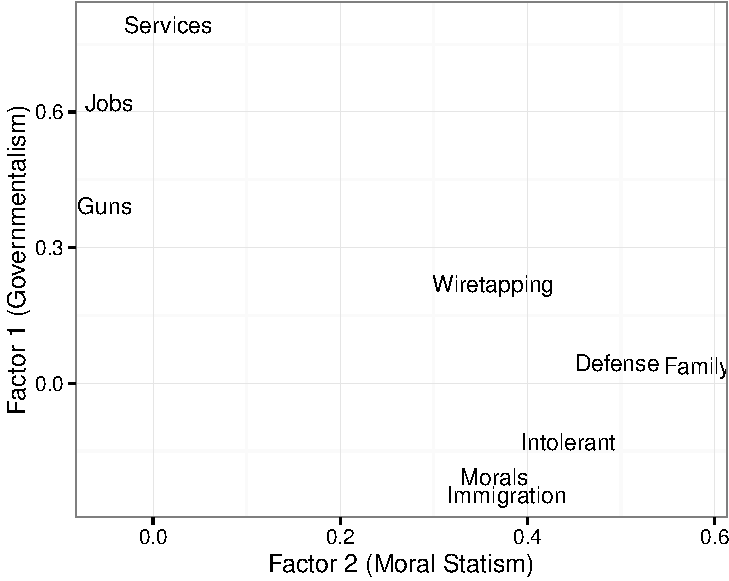
\includegraphics{figures/factorplot-1.pdf}
\caption{Factor Plot Shows Two Main Dimensions}
\end{figure}

It is important to note that we should not expect adequate overall model
fit, for two reasons. First, we are not arguing that a misarchist
dimensionality should explain so much of the variation in these nine
variables as to be a fully adequate model of them. We are only arguing
that these nine variables should contain certain identifiable,
non-trivial latent factors, consistent with Nietzsche's diagnosis, which
will explain a unique portion of Tea Party support. Second, the survey
questions refer to diverse political phenomena and likely reflect a
great deal of variation admittedly irreducible to our hypothesized
factors. At this stage of the analysis we find it satisfactory to
observe that the first two factors identified by the factor model
capture latent dimensions reflective of our argument above.\footnote{For
  \emph{N} equal to 5914, a chi-square test of the null hypothesis that
  two factors are sufficient is equal to 878 with a p-value of 0,
  suggesting that two factors are not sufficient, as we would expect.
  That said, the root mean square of the residuals is 0.05 and the
  Tucker-Lewis Index for factor reliability score is 0.8, both of which
  are near the conventional cutoffs of .05 and .9, respectively.}

What are the distributions of moral statism and governmentalism across
our sample of individuals? How do these constructs comport with what is
traditionally called conservatism? If it seems counter-intuitive for
individuals to oppose government while supporting the state, this is
only because popular conceptions of ideology have not given us the
conceptual resources to disentangle these components. Figure 2
illustrates the relationship between these two factors, across the seven
ordinal categories of the traditional ideology measure
(\emph{Conservatism}). The shaded rectangle represents misarchism:
individuals with negative scores on the \emph{Government} factor
(i.e.~libertarian) but positive scores on the \emph{Moral Statism}
factor. Figure 2 reveals a few points of interest. Firest, \emph{Moral
Statism} and \emph{Government} are negatively correlated, highlighting
the descriptive significance of disaggregating attitudes toward
government and the state. It is not even that popular conceptions of
libertarianism ignore ideological constellations ``off the diagonal'' of
correlated attitudes toward government and the state; they are
positively misleading about the direction of the correlation.\footnote{This
  is not an artifact of the factor model. The correlation plot
  illustrating correlations among all of the variables entered into the
  factor model leads to the same description (with the exception of
  \emph{Wiretapping,} which does not load strongly on either factor):
  The individual attitudes toward government are negatively correlated
  with the attitudes toward morality and the attitudes toward state
  power. See Supplementary Information.} Second, misarchism is
correlated with the traditional concept of conservatism and most of the
strong misarchists are conservatives, although misarchism is not unique
to conservatives. Indeed, the third point to note about Figure 2 is that
a degree of misarchism characterizes a non-trivial fraction of the
sample in general, including those in the center and somewhat liberal
categories of the traditional ideology variable.

\begin{figure}[htbp]
\centering
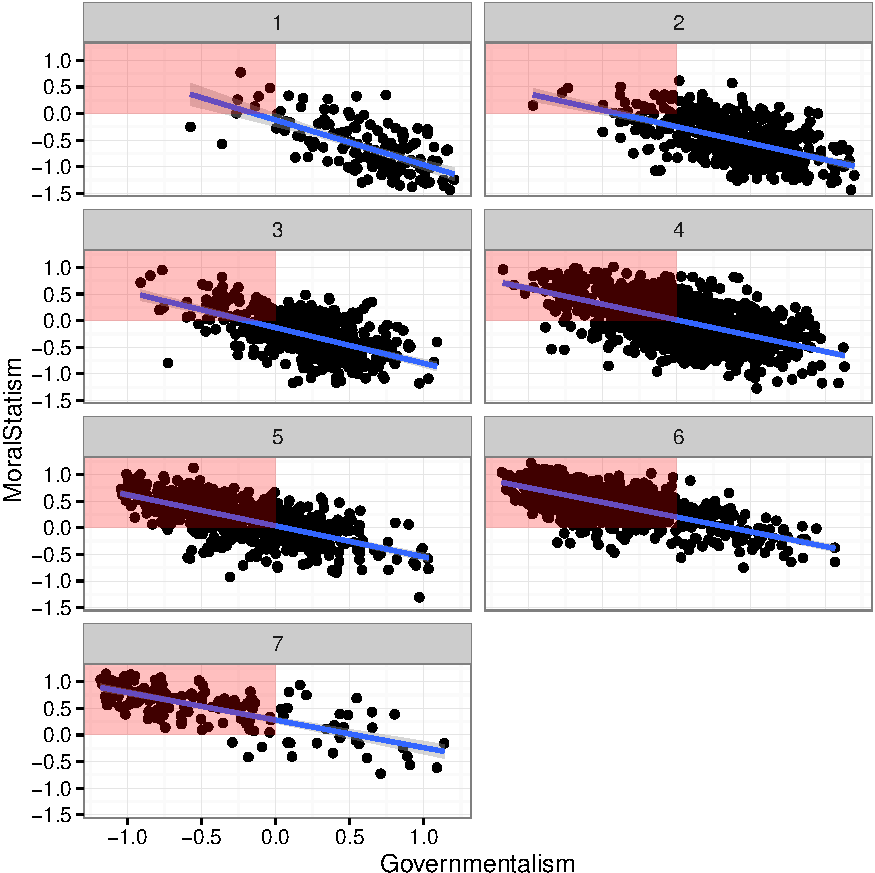
\includegraphics{figures/exploratoryplot-1.pdf}
\caption{Governmentalism and Moral Statism by Levels of Conservatism
(Shaded Rectangle Represents Misarchism)}
\end{figure}

Do the latent ideological variables of governmentalism and moral statism
help improve our understanding of support for the Tea Party? Table 1
shows results from three logistic regressions modeling the probability
that an individual will support the Tea Party. Before analysis, each
independent variable was centered to a mean of zero and divided by two
standard deviations, including the factor scores, so that all
coefficients can be interpreted as the expected change in the log-odds
of supporting the Tea Party associated with a two-standard-deviation
change in the independent variable (or a one-category change in the case
of a categorical variable). Model 1 is a baseline model including
predictors from previous research and standard demographic control
variables. Model 2 adds each of the latent variables and a term
representing the multiplicative interaction of the two. Model 3, for
reasons discussed below, is the same as Model 2 but estimated only on
the subset of respondents who identify as some degree of
``conservative'' on the traditional ideological self-placement scale.

To begin, consider the argument of Parker and Barretto that opposition
to Barack Obama is a key driver of Tea Party support. Given a typical
respondent who hypothetically drops from the 90th percentile of positive
feelings toward Obama to the 10th, we would expect the probability of
them supporting the Tea Party to change by about 13.4\% (sd=3), from a
baseline of 0.028 to 0.162 on average.\footnote{All discussion of effect
  sizes refer to 1000 simulations of Model 2 in Table 1 using the R
  package \emph{Zelig}. See (Imai, King, and Lau 2009).}

In comparison, consider the covariates capturing misarchism. Given a
typical respondent who hypothetically changes from the 10th percentile
of moral statism to the 90th when governmentalism is at its mean, we
would expect the probability of them supporting the Tea Party to change
by -0.5\% (sd = 2), from 0.068 to 0.062 on average. Given a typical
respondent who hypothetically changes from the 90th percentile of
governmentalism to the 10th when moral statism is at its mean, we would
expect the probability of them supporting the Tea Party to increase by
7.5\% (sd = 2.4), from 0.037 to 0.114 on average. To gain a sense of how
much governmentalism conditions the effect of moral statism is somewhat
more complicated. The coefficient in Model 2 for
\emph{MoralStatism:Government} reflects the estimated effect that a
two-standard-deviation increase in governmentalism has on the estimated
effect a two-standard-deviation increase in moral statism would have on
the log-odds of someone supporting the Tea Party.

Because a substantive interpretation of this interactive effect requires
us to consider multiple values for both variables at once, a graphical
illustration is most appropriate. Figure 2 plots the expected effect of
moral statism across its range for three different values of
governmentalism (-1, 0, 1). While \emph{MoralStatism} has no notable
effect on Tea Party support for individuals who moderately or strongly
support government interventions, for extreme anti-governmentalists a
hypothetical conversion from the lowest to the highest levels of moral
statism would be associated with more than a four-fold increase in the
probability of supporting the Tea Party, from less than 5\% to more than
20\%.

Consider a more typical hypothetical individual who undergoes a more
realistic ``conversion'' to a strongly misarchist ideology. For
individuals in the 90th percentile of governmentalism (strong
non-libertarians), a hypothetical shift from the 10th to the 90th
percentile of moral statism has little discernible effect on the
probability of supporting the Tea Party. The estimated change is -3.6\%
(sd = 1.8), on average. For individuals in the 10th percentile of
governmentalism (strong libertarians), a hypothetical shift from the
10th to the 90th percentile of moral statism shifts the probability of
Tea Party support by 8.1\% (sd = 3.4), from 0.081 to 0.16 on average.

In Model 2, an overall effect of misarchism on Tea Party support is
clearly discernible but relatively small, for three reasons. First,
support for the Tea Party is generally uncommon (a proportion of 0.26 in
the sample). While our estimated effect does not bring the typical
respondent close to supporting the Tea Party, this is unsurprising in
part because so few respondents support the Tea Party. Further to this
point, the simulations are based on a ``typical respondent,'' in this
case a white male who identifies with neither the Republican nor
Democratic Party, who does not watch Fox News, and who does not feel
strongly about Barack Obama. Because Tea Party support is not randomly
distributed but overwhelmingly more likely to come from conservative
individuals, it is even less surprising that the estimated effects of
misarchism for the sample as a whole are modest. Given the very low
probability a typical respondent would support the Tea Party, we should
not expect misarchism to increase the probability of Tea Party support
by very much. Indeed, in relative terms, the effect of a hypothetical
misarchist ``conversion'' is striking, roughly doubling the very low
probability a typical respondent would support the Tea Party. Second, we
have been very conservative in including a large battery of control
variables, many of which are correlated with misarchism and may measure
the same underlying
traits.\footnote{See Figure 4 in the Supplementary Information, which is a correlation plot of the independent variables capturing different dimensions of right-wing attitudes. Unsurprisingly they are all positively correlated with coefficients greater than .5.}
For the sake of hypothesis testing we have prioritised additional
control variables in order to eliminate rival hypotheses, but we note
that this has led to more conservative estimates of our hypothesized
effect.\footnote{For instance, we have chosen to include traditional ideological self-placement as a control variable to provide a more challenging test of whether misarchism affects Tea Party support independently of traditional conservatism, but if traditional ideological self-placement is just yet another measure of an underlying ideological dimension, then it may just as well have been included in the factor analysis. If ideological self-placement is included in the factor analysis and removed as a control variable in Model 2, the coefficient for the interaction term increases appreciably. With that approach, a "conversion" to moral statism for strong anti-governmentalists increases the probability of supporting the Tea Party to roughly .4. See Supplementary Information.}

To better gauge the substantive significance of misarchism for
explaining Tea Party support, it is helpful to consider conservatives
only. Considering only conservatives not only allows us to focus on the
part of the population most relevant for understanding the sources of
Tea Party support; it also allows us to explore with greater resolution
how misarchism helps to clarify otherwise indistinguishable components
of American conservatism. Model 3 in Table 1 displays results from a
regression identical to Model 2 but estimated only on the subset of
respondents who placed themselves to the right of the center (the mean)
of ideological self-placement (\emph{Conservatism}). The results are
striking. First, the coefficients for \emph{Governmentalism} and the
interaction term increase in magnitude, remaining statisticaly
significant. Importantly, this estimated effect is now sufficient to
lead the typical conservative to transition from being an unlikely to a
likely Tea Party supporter. Again it is most convenient to consider a
visualization. Figure 3 is identical to Figure 2 but now reflects Model
3. Interestingly, for moderately and strongly governmentalist
conservatives, moral statism decreases the probability of Tea Party
support from large confidence intervals encompassing the 50\% mark, to
more narrow confidence intervals making them clearly less than likely to
support the Tea Party. But for strongly anti-governmentalist
conservatives, a hypothetical conversion from the lowest to the highest
levels of moral statism would lead them toward the Tea Party, indeed
making them more likely than not to support it (the lower bound is
roughly at 50\% but the point estimate is notably higher than 50\% from
roughly .5 on the \emph{MoralStatism} factor). Therefore Model 3 shows
with a higher resolution that the concept of a misarchist interaction
between governmentalism and moral statism helps to explain why some
conservatives have gravitated into the Tea Party while others have
gravitated away from it. Considering less extreme differences in
governmentalism, for individuals in the 90th percentile of
governmentalism (strong non-libertarians), a hypothetical shift from the
10th to the 90th percentile of moral statism has a negative effect on
the probability of supporting the Tea Party. The estimated change is
-13.4\% (sd = 6.8), from 0.185 to 0.046 on average. For individuals in
the 10th percentile of governmentalism (strong libertarians), a
hypothetical shift from the 10th to the 90th percentile of moral statism
shifts the probability of Tea Party support by 8.1\% (sd = 9.3), from
0.262 to 0.358 on average.

Does the misarchist interaction of moral statism and
anti-governmentalism also drive Republican Party identification and/or
conservative identification? The answer matters for understanding how
these model results improve our understanding of American conservatism.
If a misarchist perspective is associated with Republican Party
identification or identification with conservatism in general, our
findings may only reflect a substrate of American conservatism but not
necessarily Tea Party support per se. To check this possibility, we run
two additional models similar to Model 2 but using ordinary least
squares estimation with \emph{PartyID} and \emph{Conservatism} on the
left-hand side of the model equation instead of the right-hand side. To
save space, we provide only a brief discussion of the results here, with
full model results available in the Supplementary Information. Moral
statism positively predicts and governmentalism negatively predicts
Republican identification with high levels of statistical significance,
but the coefficient for the interaction term is nearly zero and
statistically insignificant. On the other hand, considering conservative
self-identification as the dependent variable, while both moral statism
and governmentalism are again signed as expected, the interaction term
is positive and significant. These results suggest that the misarchist
interaction of moral statism and anti-governmentalism is positively
associated with Tea Party support in a fashion irreducible to simple
Republican Party identification or conservative identification. A
substantive interpretation consistent with these auxiliary models is
that the Republican Party is home to morally statist as well as
anti-government and pro-government attitudes (a ``broad church''
encompassing various forms of conservatism). On the other hand, the Tea
Party is uniquely associated with the combination of morally statist and
anti-government attitudes whereas simple ``conservatism'' is uniquely
associated with morally statist and pro-government attitudes. Because
these are not our primary, theoretically motivated arguments, caution
should be exercised in making inferences from these auxilliary models.
Nonetheless, they strengthen support for our argument and contradict the
common interpretation of Tea Party supporters as simply extreme
conservatives or extreme Republicans.

\singlespacing

\begin{table}[!htbp] \centering 
  \caption{Logistic Regressions, Tea Party Support} 
  \label{} 
\footnotesize 
\begin{tabular}{@{\extracolsep{5pt}}lccc} 
\\[-1.8ex]\hline 
\hline \\[-1.8ex] 
\\[-1.8ex] & (1) & (2) & (3)\\ 
\hline \\[-1.8ex] 
 Gender (Male) & 0.238$^{*}$ & 0.134 & 0.255$^{*}$ \\ 
  & (0.124) & (0.128) & (0.154) \\ 
  Income & $-$0.176 & $-$0.320$^{**}$ & $-$0.386$^{**}$ \\ 
  & (0.142) & (0.147) & (0.179) \\ 
  Age & $-$0.246$^{*}$ & $-$0.341$^{**}$ & $-$0.212 \\ 
  & (0.138) & (0.144) & (0.178) \\ 
  Race (White) & $-$0.338$^{**}$ & $-$0.410$^{**}$ & $-$0.510$^{**}$ \\ 
  & (0.162) & (0.168) & (0.213) \\ 
  Education & 0.114 & 0.058 & 0.134 \\ 
  & (0.153) & (0.158) & (0.195) \\ 
  Obama & $-$1.820$^{***}$ & $-$1.340$^{***}$ & $-$1.270$^{***}$ \\ 
  & (0.200) & (0.223) & (0.282) \\ 
  Authoritarianism & 0.028 & 0.054 & $-$0.124 \\ 
  & (0.142) & (0.147) & (0.174) \\ 
  BornAgain & 0.370$^{***}$ & 0.308$^{**}$ & 0.320$^{**}$ \\ 
  & (0.131) & (0.134) & (0.161) \\ 
  Religion & $-$0.040 & $-$0.024 & $-$0.044 \\ 
  & (0.152) & (0.155) & (0.190) \\ 
  PartyID (Republican) & 0.357$^{*}$ & 0.318 & 0.176 \\ 
  & (0.194) & (0.201) & (0.250) \\ 
  FoxNews & 0.776$^{***}$ & 0.700$^{***}$ & 0.735$^{***}$ \\ 
  & (0.130) & (0.133) & (0.158) \\ 
  Conservatism & 1.350$^{***}$ & 1.120$^{***}$ & 2.000$^{***}$ \\ 
  & (0.192) & (0.202) & (0.405) \\ 
  MoralStatism &  & $-$0.138 & $-$0.513 \\ 
  &  & (0.261) & (0.355) \\ 
  Governmentalism &  & $-$0.809$^{***}$ & $-$1.030$^{***}$ \\ 
  &  & (0.253) & (0.328) \\ 
  MoralStatism*Governmentalism &  & $-$1.080$^{***}$ & $-$1.210$^{***}$ \\ 
  &  & (0.316) & (0.451) \\ 
  Constant & $-$2.600$^{***}$ & $-$2.580$^{***}$ & $-$2.890$^{***}$ \\ 
  & (0.202) & (0.208) & (0.324) \\ 
 \hline \\[-1.8ex] 
Observations & 2,406 & 2,406 & 1,079 \\ 
Log Likelihood & $-$856.000 & $-$832.000 & $-$555.000 \\ 
Akaike Inf. Crit. & 1,738.000 & 1,696.000 & 1,142.000 \\ 
\hline 
\hline \\[-1.8ex] 
\textit{Note:}  & \multicolumn{3}{r}{$^{*}$p$<$0.1; $^{**}$p$<$0.05; $^{***}$p$<$0.01} \\ 
\end{tabular} 
\end{table}

\pagebreak

\doublespacing

\begin{figure}[htbp]
\centering
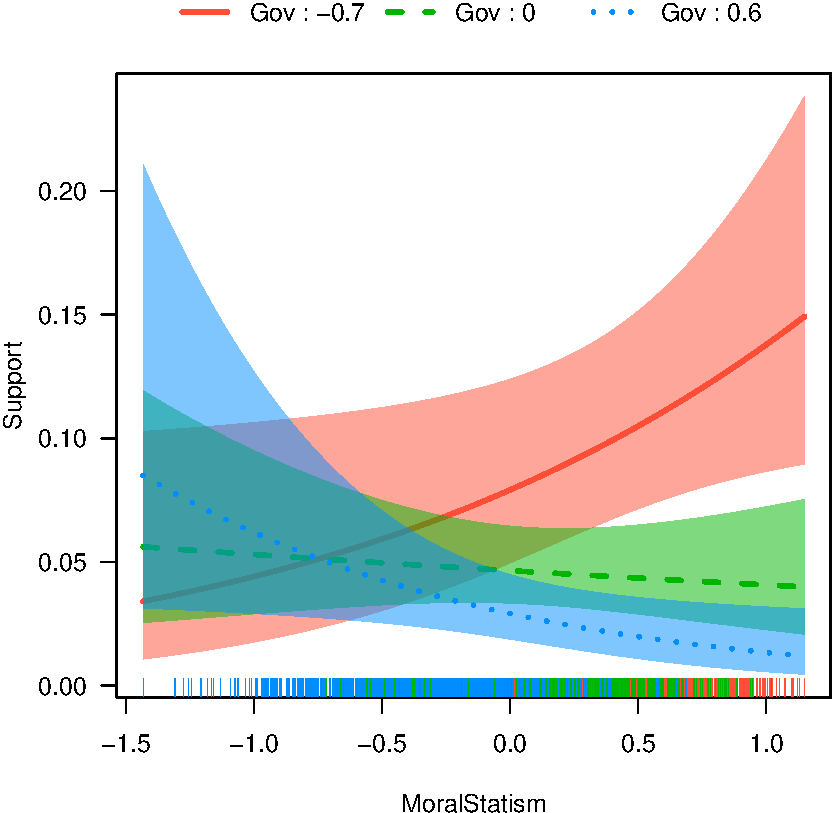
\includegraphics{figures/effect-plot1-1.pdf}
\caption{The Effect of Moral Statism Conditional on Governmentalism
(Gov)}
\end{figure}

\begin{figure}[htbp]
\centering
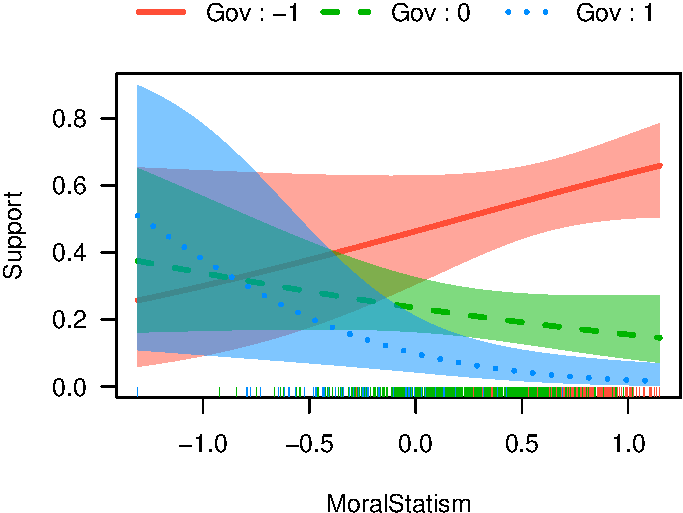
\includegraphics{figures/effect-plot2-1.pdf}
\caption{The Effect of Moral Statism Conditional on Governmentalism
(Gov) for Conservatives Only}
\end{figure}

To check the robustness of our results, we also executed a series of
additional analyses. The full results from these analyses, with
additional detail on the procedures and discussion of the results, can
be found in Supplementary Information. In short, we consider three main
threats to regression-based inferences from observational data. First,
to guard against parametric model dependence, we use a genetic matching
algorithm to identify that subset of the original dataset for which the
distribution of each covariate is optimally balanced across both
treatment and control groups (Diamond and Sekhon 2012; Sekhon 2011).
From this subset of matched pairs we estimate an average treatment
effect for those ``treated'' to the misarchist interaction. Second,
because we do not know the true model, an idiosyncratic search for
optimal model specifications can lead to bias (J. M. Montgomery and
Nyhan 2010, 4). To gauge the sensitivity of our results to model
selection, we use Bayesian Model Averaging (BMA) to calculate posterior
probabilities for all possible coefficients and models in order to
identify the most likely models and variables. Finally, another possible
problem is that listwise deletion of all observations containing missing
values may have led to biased estimates. To consider this, we employ
multiple imputation of missing values and re-estimate the regression
models. While all of these robustness checks provide additional
information and important nuance for evaluating our main argument,
overall they show that the conclusions we have drawn here are not merely
artifacts of parametric model dependence, arbitrary model selection, or
missing data.

\subsection{Conclusion}\label{conclusion}

This article demonstrates that an ideological constellation first
diagnosed by Nietzsche as ``misarchism''---a combination of
anti-government, pro-state, and moralistic attitudes---helps to predict
Tea Party support and generally improves our understanding of the
ideological nature of the Tea Party movement. In particular, we leverage
the history of political theory to provide a coherent solution to the
otherwise inexplicable combination of libertarianism and
authoritarianism which scholars have found to co-exist within the Tea
Party. While we find additional support for some previous
findings---namely, that feelings toward Obama, evangelicalism, and
exposure to Fox News are significant and robust predictors of Tea Party
support---this article is the first to provide systematic empirical
evidence that a particular ideological constellation irreducible to
libertarianism or social conservatism is a unique and notably strong
driver of Tea Party support.

Our ideological explanation also raises an interesting question about
the future of the Tea Party. If opposition to Obama were the primary
driver of Tea Party support, then we would expect Tea Party mobilization
to subside once Obama's term as President ends. If however, a
significant driver of Tea Party mobilization is a misarchist ideology,
then we would expect the Tea Party to continue to play a role in the
Republican party by supporting candidates and policies that would be in
line with misarchist beliefs long after President Obama leaves office.

There are several questions about misarchism that this study does not
answer, but are worthy of further investigation. The first is whether
misarchism represents a new ideology within the Republican party, or if
it is an ideology that has somehow been a latent feature of American
political life. If it is new, then this would raise some interesting
questions about how new ideologies form. Did the election of Obama, or a
backlash against the Stimulus Act and the Affordable Care Act, somehow
crystallize a new constellation of beliefs in the minds of a large bloc
of voters? Alternatively, was this a latent worldview held by a large
segment of the electorate that was somehow mobilized through and elite
branding campaign by Conservative activist groups such as FreedomWorks
and media outlets such as Fox News? More generally, our approach, by
thinking about the possibility of unique and diverse ideological
constellations structuring attitudes within the conventional left-right
spectrum, raises questions about what other ideological constellations
may mobilize different constituencies in American politics.

\pagebreak

\subsection{Supplementary Information}\label{supplementary-information}

\paragraph{Contents}\label{contents}

\begin{enumerate}
\def\labelenumi{\arabic{enumi}.}
\tightlist
\item
  Scree plot for factor model
\item
  Numerical factor loadings
\item
  Comparing misarchism, conservatism, and Republicanism
\item
  Including Party ID as a covariate
\item
  Estimated effects of misarchism on Party ID and Conservatism
\item
  Ideology included in factor model and removed from regression
\item
  Probabilities of covariate inclusion from Bayesian Model Averaging
\item
  Expected value of coefficients from Bayesian Model Averaging
\item
  Pooled regression results after multiple imputation
\item
  Multiple imputation diagnostics
\end{enumerate}

\begin{figure}[htbp]
\centering
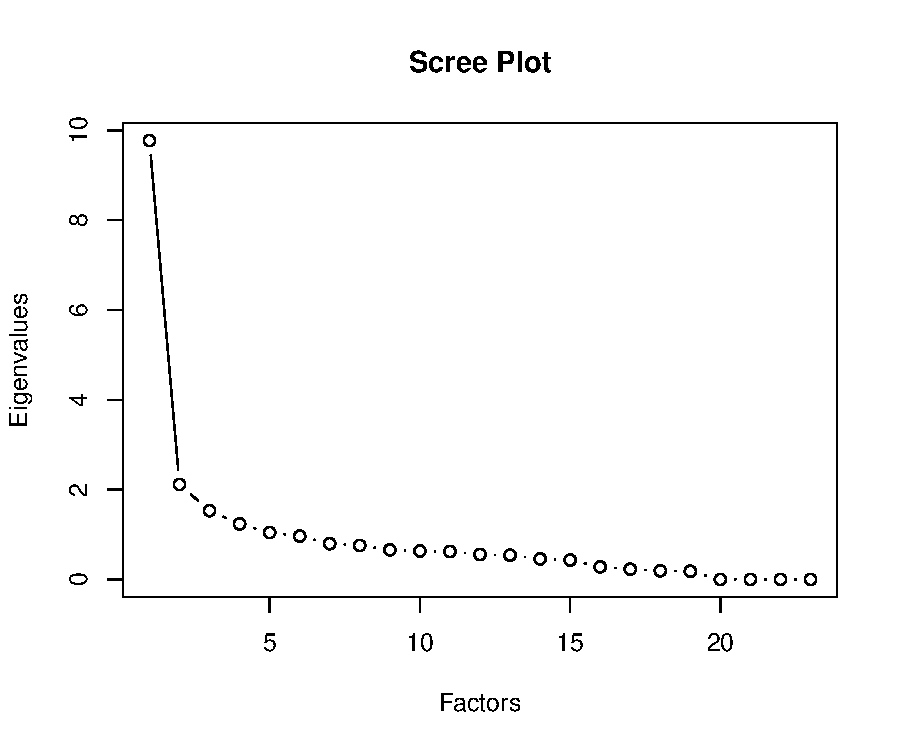
\includegraphics{figures/scree-1.pdf}
\caption{Scree Plot for Determining Number of Factors}
\end{figure}

\clearpage

\begin{table}[ht]
\centering
\begin{tabular}{rrr}
  \hline
 & Governmentalism & Moral Statism \\ 
  \hline
Family & 0.03 & 0.59 \\ 
  Guns & 0.40 & -0.05 \\ 
  Intolerant & -0.12 & 0.44 \\ 
  Morals & -0.22 & 0.36 \\ 
  Wiretapping & 0.21 & 0.35 \\ 
  Defense & 0.04 & 0.49 \\ 
  Services & 0.78 & 0.01 \\ 
  Immigration & -0.24 & 0.38 \\ 
  Jobs & 0.61 & -0.04 \\ 
   \hline
\end{tabular}
\caption{Factor Loadings} 
\label{Factor Loadings From Main Factor Analysis}
\end{table}

\begin{figure}[htbp]
\centering
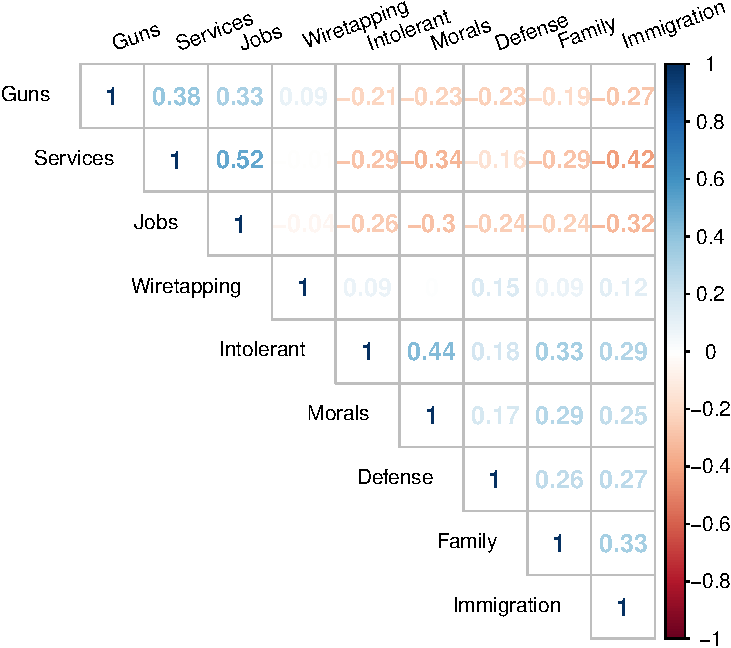
\includegraphics{figures/corrplot1-1.pdf}
\caption{Correlation Plot for Variables Included in Factor Model}
\end{figure}

\begin{figure}[htbp]
\centering
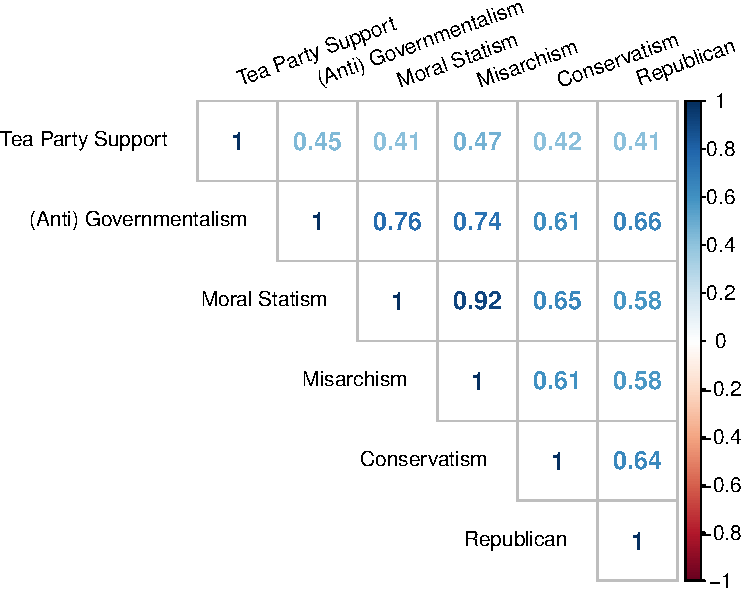
\includegraphics{figures/corrplot2-1.pdf}
\caption{Correlation Plot for Different Measures of Right-Wing Politics
(Governmentalism Reversed for Ease of Interpretation)}
\end{figure}

\clearpage

\begin{table}[!htbp] \centering 
  \caption{Alternative Dependent Variables for Model 2} 
  \label{} 
\footnotesize 
\begin{tabular}{@{\extracolsep{5pt}}lcc} 
\\[-1.8ex]\hline 
\hline \\[-1.8ex] 
 & \multicolumn{2}{c}{\textit{Dependent variable:}} \\ 
\cline{2-3} 
\\[-1.8ex] & PartyID (Republican) & Conservatism \\ 
\\[-1.8ex] & (1) & (2)\\ 
\hline \\[-1.8ex] 
 Gender (Male) & $-$0.006 & 0.008 \\ 
  & (0.013) & (0.014) \\ 
  Income & 0.032$^{**}$ & $-$0.003 \\ 
  & (0.015) & (0.016) \\ 
  Age & $-$0.057$^{***}$ & 0.025 \\ 
  & (0.014) & (0.016) \\ 
  Race (White) & 0.076$^{***}$ & $-$0.058$^{***}$ \\ 
  & (0.015) & (0.017) \\ 
  Education & 0.044$^{***}$ & $-$0.024 \\ 
  & (0.015) & (0.017) \\ 
  Obama & $-$0.545$^{***}$ & $-$0.103$^{***}$ \\ 
  & (0.020) & (0.025) \\ 
  Authoritarianism & $-$0.029$^{**}$ & 0.039$^{**}$ \\ 
  & (0.015) & (0.016) \\ 
  BornAgain & 0.016 & 0.030$^{*}$ \\ 
  & (0.014) & (0.015) \\ 
  Religion & 0.001 & 0.038$^{**}$ \\ 
  & (0.015) & (0.017) \\ 
  PartyID (Republican) &  & 0.321$^{***}$ \\ 
  &  & (0.022) \\ 
  FoxNews & 0.039$^{**}$ & 0.059$^{***}$ \\ 
  & (0.015) & (0.017) \\ 
  Conservatism & 0.256$^{***}$ &  \\ 
  & (0.018) &  \\ 
  MoralStatism & $-$0.001 & 0.259$^{***}$ \\ 
  & (0.024) & (0.026) \\ 
  Governmentalism & $-$0.103$^{***}$ & $-$0.100$^{***}$ \\ 
  & (0.023) & (0.026) \\ 
  MoralStatism*Governmentalism & 0.025 & 0.044 \\ 
  & (0.026) & (0.029) \\ 
  Constant & $-$0.051$^{***}$ & $-$0.009 \\ 
  & (0.019) & (0.022) \\ 
 \hline \\[-1.8ex] 
Observations & 2,406 & 2,406 \\ 
R$^{2}$ & 0.674 & 0.523 \\ 
Adjusted R$^{2}$ & 0.673 & 0.521 \\ 
Residual Std. Error (df = 2391) & 0.305 & 0.342 \\ 
F Statistic (df = 14; 2391) & 354.000$^{***}$ & 187.000$^{***}$ \\ 
\hline 
\hline \\[-1.8ex] 
\textit{Note:}  & \multicolumn{2}{r}{$^{*}$p$<$0.1; $^{**}$p$<$0.05; $^{***}$p$<$0.01} \\ 
\end{tabular} 
\end{table}

\clearpage

\begin{table}[!htbp] \centering 
  \caption{Including Ideology in Factor Model and Removing From Regression Model} 
  \label{} 
\footnotesize 
\begin{tabular}{@{\extracolsep{5pt}}lc} 
\\[-1.8ex]\hline 
\hline \\[-1.8ex] 
 & \multicolumn{1}{c}{\textit{Dependent variable:}} \\ 
\cline{2-2} 
\\[-1.8ex] & Tea Party Support \\ 
\hline \\[-1.8ex] 
 Gender (Male) & 0.128 \\ 
  & (0.128) \\ 
  Income & $-$0.321$^{**}$ \\ 
  & (0.147) \\ 
  Age & $-$0.379$^{***}$ \\ 
  & (0.144) \\ 
  Race (White) & $-$0.453$^{***}$ \\ 
  & (0.167) \\ 
  Education & 0.058 \\ 
  & (0.158) \\ 
  Obama & $-$1.300$^{***}$ \\ 
  & (0.222) \\ 
  Authoritarianism & 0.028 \\ 
  & (0.147) \\ 
  BornAgain & 0.296$^{**}$ \\ 
  & (0.134) \\ 
  Religion & $-$0.013 \\ 
  & (0.154) \\ 
  PartyID (Republican) & 0.435$^{**}$ \\ 
  & (0.198) \\ 
  FoxNews & 0.707$^{***}$ \\ 
  & (0.133) \\ 
  MoralStatism & 0.708$^{**}$ \\ 
  & (0.283) \\ 
  Governmentalism & $-$0.799$^{***}$ \\ 
  & (0.268) \\ 
  MoralStatism*Governmentalism & $-$1.230$^{***}$ \\ 
  & (0.332) \\ 
  Constant & $-$2.520$^{***}$ \\ 
  & (0.206) \\ 
 \hline \\[-1.8ex] 
Observations & 2,406 \\ 
Log Likelihood & $-$835.000 \\ 
Akaike Inf. Crit. & 1,701.000 \\ 
\hline 
\hline \\[-1.8ex] 
\textit{Note:}  & \multicolumn{1}{r}{$^{*}$p$<$0.1; $^{**}$p$<$0.05; $^{***}$p$<$0.01} \\ 
\end{tabular} 
\end{table}

Individuals characterized by the highest observed levels of moral
statism also in the 90th percentile of anti-governmentalism (below a
value of -.7 on the governmentalism factor) have a probability of
supporting the Tea Party around 40\%. To be more precise, moving from
minimum to maxium moral statism while in the 10th percentile of
governmentalism increases the probability of supporting the Tea Party by
.39 (sd=.07) more than it would in the 90th percentile of
governmentalism, from .01 (sd=.00) to .42, (sd=.07) rather than .05
(sd=.02) to .03 (sd=.02).

\clearpage

\subsubsection{Bayesian Model Averaging}\label{bayesian-model-averaging}

Regression results such as those presented above are sometimes sensitive
to minor differences in model specification, such as including or
excluding one variable. One risk is publication bias, if researchers
prefer models that confirm their hypotheses. Another is loss of
efficiency if too many unnecessary variables are included. Finally, an
\emph{ad hoc} approach leads to incomplete representations of model
uncertainty (J. M. Montgomery and Nyhan 2010, 4).

In particular, a version of the R package \emph{BMA} modified by
Mongtomery and Nyhan was used to search over the entire model space of
Model 2.\footnote{The analysis was conducted using the
  \emph{bic.glmMN()} function, which is a version of the
  \emph{bic.glm()} function in the R package \emph{BMA}. See (Raftery et
  al. 2015) and (J. M. Montgomery and Nyhan 2010)} The analysis uses
uniform priors for all independent variables and the only restriction is
that the interaction term and its two component variables are required
to enter or not enter models together.\footnote{Options were set to be
  least restrictive. No Occam's Window was used to narrow the models
  selected by the initial leap algorithm run over the entire model space
  and, following Montgomery and Nyhan (pp.~21), the number of best
  models of each size returned by the leaps algorithm was set to 100,000}
In the end, 8,192 models were selected.

The results show that the misarchist terms are highly robust to model
selection, with a posterior probability of inclusion equal to 100\% (one
minus the cumulative posterior probability of all models excluding
them). The expected value of the coefficient for \emph{MoralStatism} is
-0.16 (sd=.26), suggesting it has no independent effect. for
\emph{Governmentalism} it is -.76 (sd=.25), and for the interaction term
it is -1.07 (sd=.31). \emph{Obama}, \emph{FoxNews}, and
\emph{Conservatism} also had probabilities of inclusion equal to 100\%
with signs consistent with Model 2. \emph{Age}, \emph{Race}, and
\emph{BornAgain} had probabilities of inclusion greater than 25\% but
did not show expected values statistically distinguishable from zero.
All other variables had probabilities of inclusion less than 50\%. More
detailed graphical information is reported in Supplementary Information.

In the main models reported above, we have consciously chosen to include
a large number of control variables because we are presently most
concerned with testing our hypotheses and ruling out rival hypotheses.
BMA provides further evidence that the models presented above likely
contain superfluous independent variables. Though we believe it is best
to rely primarily on the conservative estimates reported above, we
briefly report how our coefficients of interest would change under
different specifications suggested by the BMA. In a model with just
those variables found to be the most robust to model selection
(\emph{Conservatism}, \emph{Fox News}, \emph{Obama},
\emph{MoralStatism}, and \emph{Governmentalism}), moving from 10th
percentile of \emph{MoralStatism} to 90th within the 10th percentile of
\emph{Governmentalism} (strong libertarian), is associated with the
probablitity of supporting the Tea Party increasing about 9\% (sd=.03)
from .09 (sd=.03) to .19 (sd=.03). Thus, the results from Bayesian Model
Averaging suggest the main results reported above are robust to model
selection.

\begin{figure}[htbp]
\centering
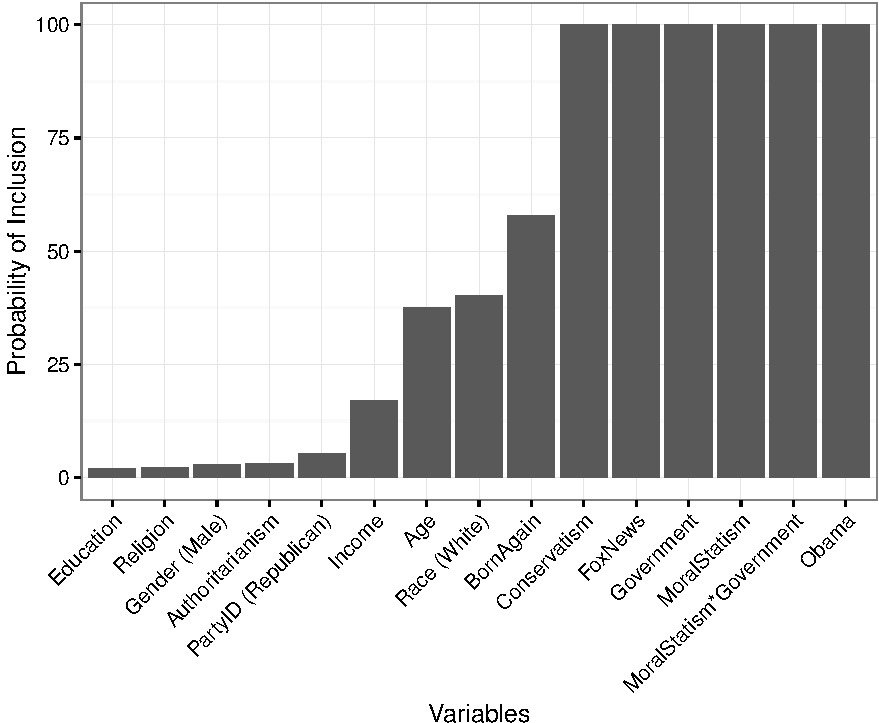
\includegraphics{figures/bma2-1.pdf}
\caption{Inclusion Probabilites from Bayesian Model Averaging}
\end{figure}

\clearpage

\begin{figure}[htbp]
\centering
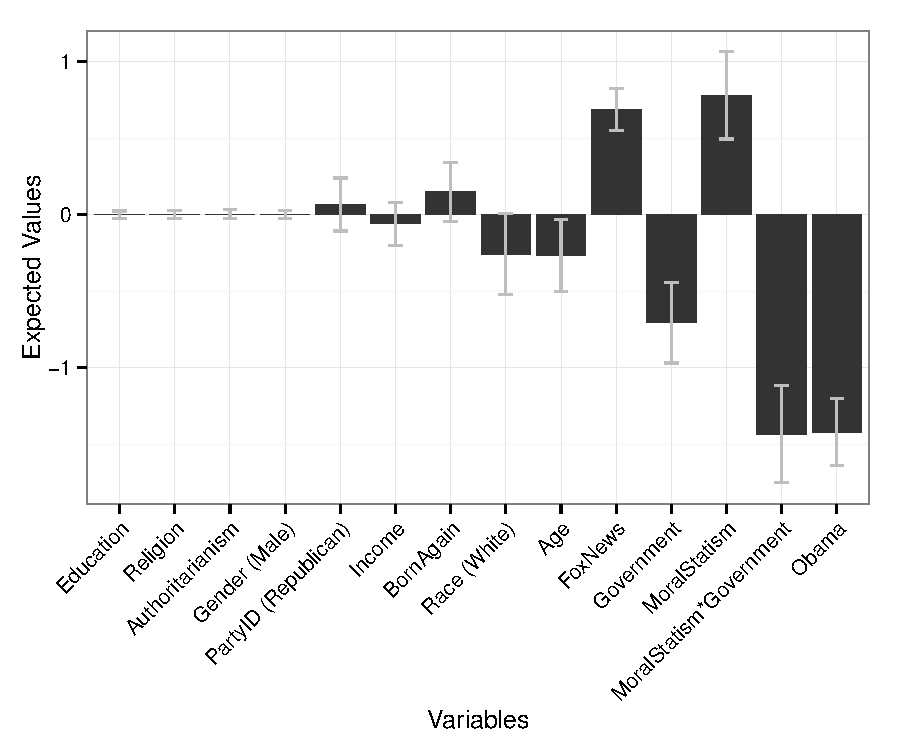
\includegraphics{figures/bma3-1.pdf}
\caption{Expected Values from Bayesian Model Averaging}
\end{figure}

\clearpage

\subsubsection{Multiple Imputation}\label{multiple-imputation}

In particular, if relative misarchists were more (or less) likely to
respond to certain questions than other respondents, we may have
over-estimated (or under-estimated) the true partial correlation between
our misarchist terms and Tea Party support. Multiple imputation refers
to the process of using the information from observed variables to infer
the most likely values for all missing cells. The process finishes by
producing a set of new datasets each of which samples from the
predictive distribution to assign most likely values to each missing
cell. After multiple imputation, the models discussed above are
re-estimated on each imputed dataset and the results are combined using
``Rubin's rules.'' Specifically, we use the R package \emph{Amelia}
(Honaker, King, and Blackwell 2008) to generate 10 versions of the ANES
dataset with missing values imputed and \emph{Zelig} to obtain pooled
regression results. The multiple imputation algorithm only assumes that
missing values are ``missing at random,'' not necessarily ``missing
completely at random.'' In this context, ``missing at random'' only
means that missingness is dependent on the observed variables.

After pooling the results, the estimates remain substantially the same.
\emph{MoralStatism}, \emph{Governmentalism}, and the interaction term
remain signed as in Model 2 with high statistical significance (.98,
p\textless{}.00; -.68, p\textless{}.00; -1.35, p\textless{}.00,
respectively). \emph{FoxNews} and \emph{BornAgain} also remain
substantially the same. Graphical diagnostics for overimputation,
dispersion, and comparing pre- and post-imputation densities for our
main variables suggest no problems or anomolies in the imputation
procedures. \clearpage

\begin{table}[ht]
\centering
\begin{tabular}{rrrrr}
  \hline
 & Value & Std. Error & t-stat & p-value \\ 
  \hline
(Intercept) & -2.07 & 0.11 & -18.21 & 0.00 \\ 
  Gender (Female) & -0.10 & 0.09 & -1.21 & 0.23 \\ 
  Income & -0.27 & 0.11 & -2.54 & 0.01 \\ 
  Age & -0.22 & 0.10 & -2.27 & 0.02 \\ 
  Race (White) & -0.29 & 0.11 & -2.77 & 0.01 \\ 
  Education & -0.02 & 0.11 & -0.21 & 0.83 \\ 
  Obama & -0.95 & 0.14 & -6.92 & 0.00 \\ 
  Authoritarianism & 0.10 & 0.10 & 0.97 & 0.33 \\ 
  BornAgain & -0.26 & 0.09 & -2.76 & 0.01 \\ 
  Religion & 0.03 & 0.10 & 0.32 & 0.75 \\ 
  PartyID (Republican) & 0.21 & 0.13 & 1.61 & 0.11 \\ 
  FoxNews & 0.71 & 0.10 & 7.40 & 0.00 \\ 
  Conservatism & 0.98 & 0.13 & 7.46 & 0.00 \\ 
  MoralStatism & 0.07 & 0.20 & 0.35 & 0.73 \\ 
  Governmentalism & -0.86 & 0.18 & -4.70 & 0.00 \\ 
  MoralStatism*Governmentalism & -0.85 & 0.21 & -3.96 & 0.00 \\ 
   \hline
\end{tabular}
\caption{Pooled Logistic Regression Results From 10 Multiple Imputations} 
\end{table}

\clearpage

\begin{figure}[htbp]
\centering
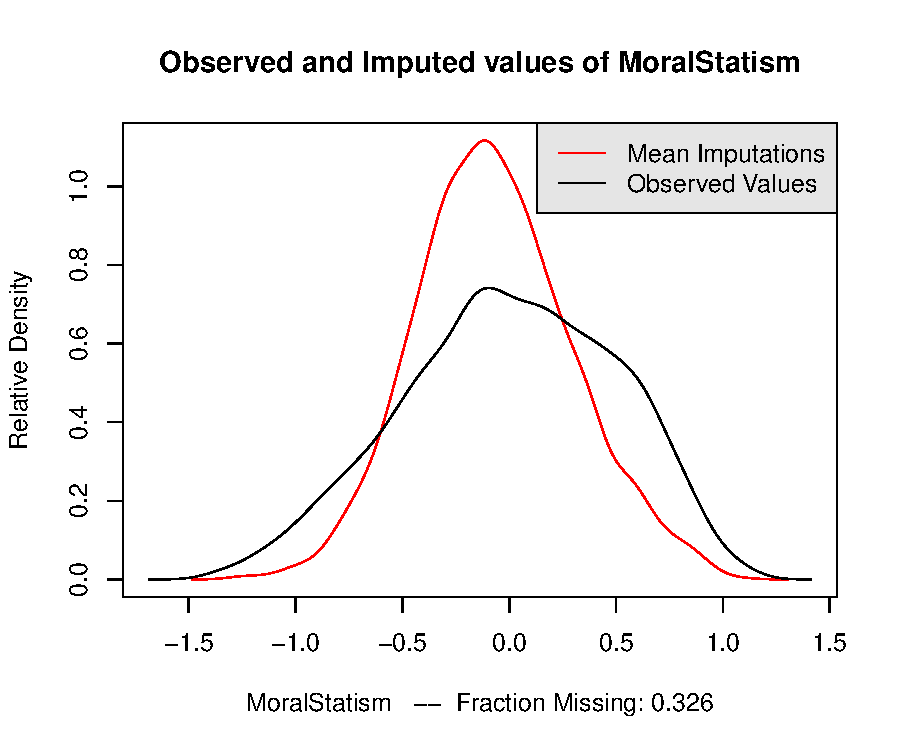
\includegraphics{figures/missing2-1.pdf}
\caption{Distributions Before and After Multiple Imputation (1)}
\end{figure}

\begin{figure}[htbp]
\centering
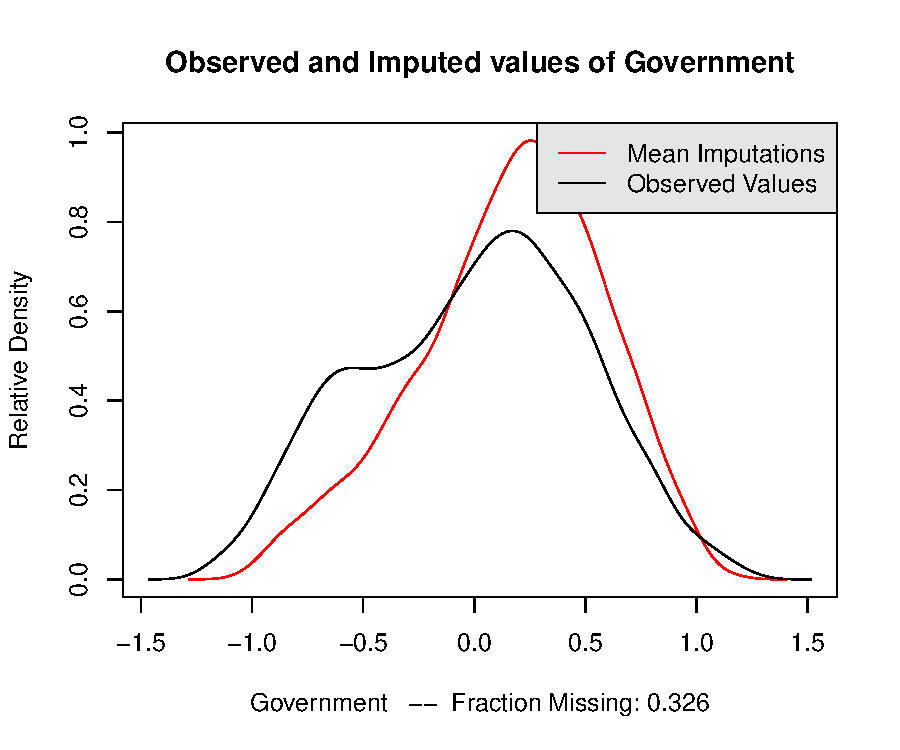
\includegraphics{figures/missing3-1.pdf}
\caption{Distributions Before and After Multiple Imputation (2)}
\end{figure}

\clearpage

\begin{figure}[htbp]
\centering
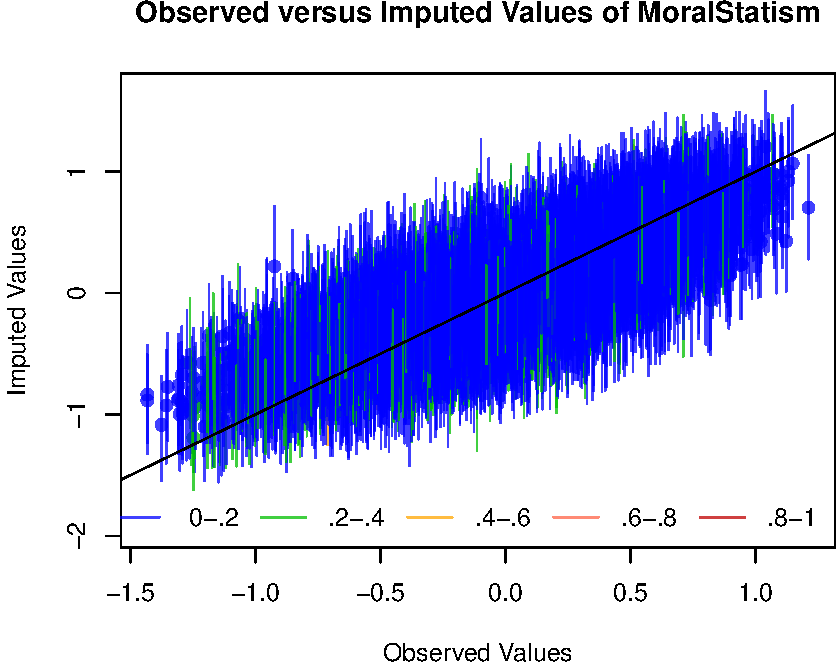
\includegraphics{figures/missing4-1.pdf}
\caption{Diagnostic Plot for Overimputation (1)}
\end{figure}

\begin{figure}[htbp]
\centering
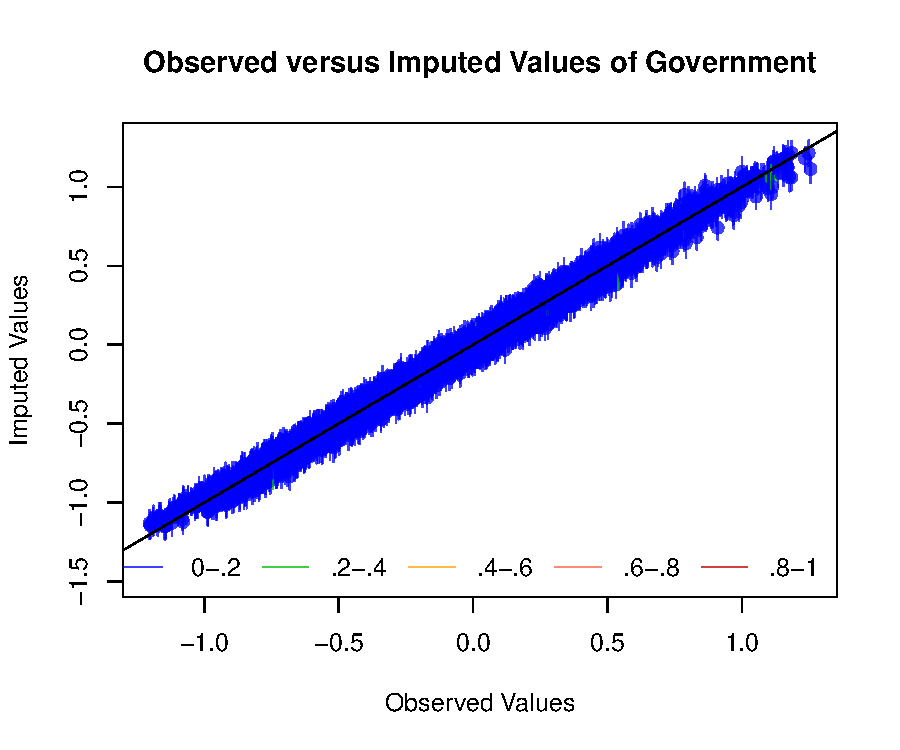
\includegraphics{figures/missing5-1.pdf}
\caption{Diagnostic Plot for Overimputation (2)}
\end{figure}

\clearpage

\begin{figure}[htbp]
\centering
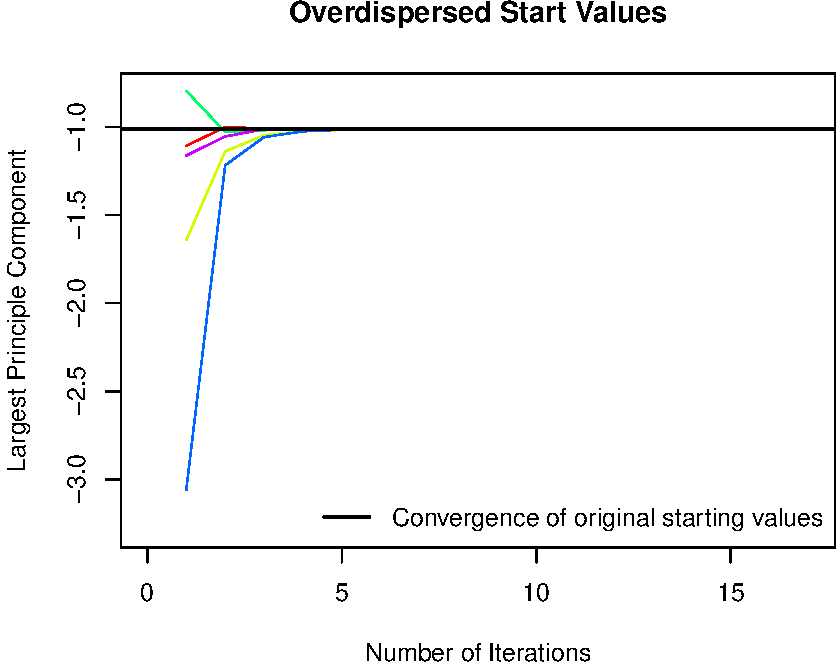
\includegraphics{figures/missing6-1.pdf}
\caption{Diagnostic Plot for Dispersion}
\end{figure}

\subsubsection{Matching and Sensitivity}\label{matching-and-sensitivity}

The algorithm obtains the matched pairs of those ``treated'' and not
treated to governmentalism and moral statism which are otherwise
optimally balanced in the propensity to be treated. The average
treatment effect for the treated obtained from this subset will
approximate that which we would obtain from a randomized experiment,
unless some unobserved factor shapes the propensity to be treated.
Although the possibility of omitted variables can never be ruled out, we
can quantify the sensitivity of these matching estimates to some
potential unobserved source of bias. Thus, we also report sensitivity
bounds as developed by Rosenbaum (1988).

We generate matching estimates for the effect of governmentalism and the
interaction term, one at a time, using one-to-one genetic matching with
replacement. We ignore moral statism because the main analyses suggest
it does not have an independent effect. In each case, ``treatment'' is
defined as having a value above the sample mean of the variable of
interest. For each estimate, we balance on all covariates in Model 2
except the two components of the interaction term and including the
treatment variable's propensity scores with respect to those covariates.
We do not balance on the components of the interaction term, or the
interaction term itself, because this would remove the covariation of
governmentalism and moral statism the effect of which we wish to test,
but we do include the components and the interaction term as covariates.

The average treatment effect on those ``treated'' with greater than the
mean level of governmentalism is -0.025, with a standard error of 0.012
(p=.04). The Rosenbaum bounds for this effect suggest that for it to
become statistically insignificant at the 95\% confidence level, the
odds of differential assignment to treatment due to an unobserved factor
would have to be about 1.45. The average treatment effect on those
``treated'' with greater than the mean level of the interaction term is
-0.022, with a standard error of 0.01 and a (p=.03). The Rosenbaum
bounds for this effect suggest that for it to become statistically
insignificant at the 95\% confidence level, the odds of differential
assignment to treatment due to an unobserved factor would have to be
about 1.39. The direction and statistical significance of the key
relationship in Model 2 (the interaction term), and one of its
independent components (governmentalism), do not appear to be spurious
artifacts of systematic assignment into treatment from any of the other
main covariates making individuals more likely to be misarchist.

\clearpage

\subsection{References}\label{references}

\setlength{\parindent}{-0.2in} \setlength{\leftskip}{0.2in}
\setlength{\parskip}{8pt} \vspace*{-0.2in} \noindent

\hyperdef{}{ref-abramowitzux5fgrandux5f2012}{\label{ref-abramowitzux5fgrandux5f2012}}
Abramowitz, Alan I. 2012. ``Grand Old Tea Party: Partisan Polarization
and the Rise of the Tea Party Movement.'' In \emph{Steep: The
Precipitous Rise of the Tea Party}, Berkeley, California: University of
California Press, 195--211.

\hyperdef{}{ref-althusserux5fideologyux5f1971}{\label{ref-althusserux5fideologyux5f1971}}
Althusser, Louis. 1971. ``Ideology and Ideological State Apparatuses
(Notes Towards an Investigation).'' In \emph{Lenin and Philosophy and
Other Essays.}, New York: Monthly Review Press.

\hyperdef{}{ref-arceneauxux5fwhoux5f2012}{\label{ref-arceneauxux5fwhoux5f2012}}
Arceneaux, Kevin, and Stephen P. Nicholson. 2012. ``Who Wants to Have a
Tea Party? The Who, What, and Why of the Tea Party Movement.'' \emph{PS:
Political Science \& Politics} 45(04): 700--710.

\hyperdef{}{ref-baileyux5fteaux5f2012}{\label{ref-baileyux5fteaux5f2012}}
Bailey, Michael A., Jonathan Mummolo, and Hans Noel. 2012. ``Tea Party
Influence: A Story of Activists and Elites.'' \emph{American Politics
Research} 40(5): 769--804.

\hyperdef{}{ref-berletux5freframingux5f2012}{\label{ref-berletux5freframingux5f2012}}
Berlet, Chip. 2012. ``Reframing Populist Resentments in the Tea Party
Movement.'' In \emph{Steep: The Precipitous Rise of the Tea Party}, eds.
Christine Trost and Lawrence Rosenthal. Berkeley, California: University
of California Press, 42--66.

\hyperdef{}{ref-Bradberry:2014eq}{\label{ref-Bradberry:2014eq}}
Bradberry, Leigh A, and Gary C Jacobson. 2014. ``The Tea Party and the
2012 presidential election.'' \emph{Electoral Studies}.
\href{Online only: http://bit.ly/1DsIbv9}{Online only: http://bit.ly/1DsIbv9}.

\hyperdef{}{ref-brennanux5flibertarianismux5f2012}{\label{ref-brennanux5flibertarianismux5f2012}}
Brennan, Jason. 2012. \emph{Libertarianism: What Everyone Should Know}.
Oxford: Oxford University Press.

\hyperdef{}{ref-brysonux5fpoliticalux5f1968}{\label{ref-brysonux5fpoliticalux5f1968}}
Bryson, Maurice C., and William R. McDill. 1968. ``The Political
Spectrum: A Bi-Dimensional Approach.'' \emph{Rampart Journal of
Individualist Thought} 4(2).
\url{https://mises.org/journals/rampart/Rampart_summer1968.pdf} (July
21, 2015).

\hyperdef{}{ref-burackux5fintroduction:ux5f2012}{\label{ref-burackux5fintroduction:ux5f2012}}
Burack, Cynthia, and R. Claire Snyder-Hall. 2012. ``Introduction:
Right-Wing Populism and the Media.'' \emph{New Political Science} 34(4):
439--54. \url{http://dx.doi.org/10.1080/07393148.2012.729736} (July 28,
2014).

\hyperdef{}{ref-campbell1980american}{\label{ref-campbell1980american}}
Campbell, Angus, Philip E Converse, Warren E Miller, and Donald E
Stokes. 1960. \emph{The American Voter}. Chicago: University of Chicago
Press.

\hyperdef{}{ref-Carmines:2014wp}{\label{ref-Carmines:2014wp}}
Carmines, Edward G, and Nicholas J D'Amico. 2014. ``The New Look in
Political Ideology Research.'' \emph{Annual Review of Political Science}
18(1): 205--16.

\hyperdef{}{ref-Converse:1964bk}{\label{ref-Converse:1964bk}}
Converse, Philip E. 1964. ``The Nature of Belief Systems in Mass
Publics.'' In \emph{Ideology and Its Discontents}, ed. David E Apter.
New York: The Free Press of Glencoe.

\hyperdef{}{ref-courserux5fteaux5f2012}{\label{ref-courserux5fteaux5f2012}}
Courser, Zachary. 2012. ``The Tea `Party' as a Conservative Social
Movement.'' \emph{Society} 49(1): 43--53.
\url{http://link.springer.com/article/10.1007/s12115-011-9501-0} (July
28, 2014).

\hyperdef{}{ref-Diamond:2012jo}{\label{ref-Diamond:2012jo}}
Diamond, Alexis, and Jasjeet S Sekhon. 2012. ``Genetic Matching for
Estimating Causal Effects: A General Multivariate Matching Method for
Achieving Balance in Observational Studies.'' \emph{Review of Economics
and Statistics} 95(3): 932--45.

\hyperdef{}{ref-dischux5fteaux5f2011}{\label{ref-dischux5fteaux5f2011}}
Disch, Lisa. 2011. ``Tea Party Movement: The American `Precariat'?''
\emph{Representation} 47(2): 123--35.
\url{http://dx.doi.org/10.1080/00344893.2011.581057} (July 28, 2014).

\hyperdef{}{ref-ellis2007symbolic}{\label{ref-ellis2007symbolic}}
Ellis, Christopher, and James A Stimson. 2007. ``On symbolic
conservatism in America.'' In \emph{Annual Meetings of the American
Political Science Association. Chicago, IL},

\hyperdef{}{ref-Ellis:2009kp}{\label{ref-Ellis:2009kp}}
---------. 2009. ``Symbolic ideology in the American electorate.''
\emph{Electoral Studies} 28(3): 388--402.
\url{http://linkinghub.elsevier.com/retrieve/pii/S0261379409000468}.

\hyperdef{}{ref-eysenckux5fpsychologyux5f1960}{\label{ref-eysenckux5fpsychologyux5f1960}}
Eysenck, Hans J. 1960. \emph{The Psychology of Politics}. Piscataway,
New Jersey: Transaction Publishers.

\hyperdef{}{ref-Fabrigar:1999cq}{\label{ref-Fabrigar:1999cq}}
Fabrigar, Leandre R, Duane T Wegener, Robert C MacCallum, and Erin J
Strahan. 1999. ``Evaluating the use of exploratory factor analysis in
psychological research.'' \emph{Psychological Methods} 4(3): 272--99.

\hyperdef{}{ref-Feldman:2013ie}{\label{ref-Feldman:2013ie}}
Feldman, Stanley. 2013. ``Political Ideology.'' In ed. Jack S. Levy
Leonie Huddy David O. Sears. Oxford University Press, USA.
\url{http://www.oxfordhandbooks.com/view/10.1093/oxfordhb/9780199760107.001.0001/oxfordhb-9780199760107-e-019}.

\hyperdef{}{ref-Feldman:2014ea}{\label{ref-Feldman:2014ea}}
Feldman, Stanley, and Christopher Johnston. 2014. ``Understanding the
Determinants of Political Ideology: Implications of Structural
Complexity.'' \emph{Political Psychology} 35(3): 337--58.
\url{http://onlinelibrary.wiley.com.libproxy.temple.edu/doi/10.1111/pops.12055/full}.

\hyperdef{}{ref-foucaultux5fgovernmentalityux5f1991}{\label{ref-foucaultux5fgovernmentalityux5f1991}}
Foucault, Michel. 1991. ``Governmentality.'' In \emph{The Foucault
Effect: Studies in Governmentality}, eds. Graham Burchell, Colin Gordon,
and Peter Miller. Chicago: University of Chicago Press, 87--104.

\hyperdef{}{ref-freedenux5fideologyux5f2003}{\label{ref-freedenux5fideologyux5f2003}}
Freeden, Michael. 2003. \emph{Ideology: A Very Short Introduction}.
Oxford: Oxford University Press.

\hyperdef{}{ref-gordonux5fgovernmentalux5f1991}{\label{ref-gordonux5fgovernmentalux5f1991}}
Gordon, Colin. 1991. ``Governmental Rationality: An Introduction.'' In
\emph{The Foucault Effect: Studies in Governmentality}, eds. Graham
Burchell, Colin Gordon, and Peter Miller. Chicago: University Of Chicago
Press, 1--52.

\hyperdef{}{ref-gorenux5fvoterux5f2013}{\label{ref-gorenux5fvoterux5f2013}}
Goren, Paul. 2013. \emph{On Voter Competence}. Oxford: Oxford University
Press.

\hyperdef{}{ref-Graham:2009er}{\label{ref-Graham:2009er}}
Graham, Jesse, Jonathan Haidt, and Brian A Nosek. 2009. ``Liberals and
conservatives rely on different sets of moral foundations.''
\emph{Journal of Personality and Social Psychology} 96(5): 1029--46.
\url{http://psycnet.apa.org/journals/psp/96/5/1029.html}.

\hyperdef{}{ref-Haidt:2012vc}{\label{ref-Haidt:2012vc}}
Haidt, Jonathan. 2012. \emph{The Righteous Mind: Why Good People are
Divided by Politics and Religion}. New York: Pantheon.

\hyperdef{}{ref-heywoodux5fpoliticalux5f2007}{\label{ref-heywoodux5fpoliticalux5f2007}}
Heywood, Andrew. 2007. \emph{Political Ideologies}. 4th ed. Basingstoke:
Palgrave Macmillan.

\hyperdef{}{ref-hoffmanux5fbeyondux5f1995}{\label{ref-hoffmanux5fbeyondux5f1995}}
Hoffman, John. 1995. \emph{Beyond the State: An Essay in Interpretation:
An Introductory Critique}. Cambridge, UK: Polity Press.

\hyperdef{}{ref-Honaker:2008vv}{\label{ref-Honaker:2008vv}}
Honaker, James, Gary King, and Matthew Blackwell. 2008. ``Amelia II: A
Program for Missing Data.'' \emph{Journal of Statistical Software}
45(i07).

\hyperdef{}{ref-huxleyux5fadministrativeux5f1871}{\label{ref-huxleyux5fadministrativeux5f1871}}
Huxley, Thomas. 1871. ``Administrative Nihilism (1871).''
\url{http://aleph0.clarku.edu/huxley/CE1/AdNil.html} (April 12, 2014).

\hyperdef{}{ref-ZeligEveryonesSt:2009ts}{\label{ref-ZeligEveryonesSt:2009ts}}
Imai, Kosuke, Gary King, and Olivia Lau. 2009. ``Zelig: Everyone's
Statistical Software.'' \url{http://gking.harvard.edu/zelig}.

\hyperdef{}{ref-publicux5freligionux5fresearchux5finstituteux5fsurvey2013}{\label{ref-publicux5freligionux5fresearchux5finstituteux5fsurvey2013}}
Jones, Robert P, Daniel Cox, and Juhem Navarro-Rivera. 2013. ``2013
American Values Survey: In Search of Libertarians in America.''
\emph{Public Religion Research Institute}.
\url{http://publicreligion.org/research/2013/10/2013-american-values-survey/}
(September 18, 2014).

\hyperdef{}{ref-karpowitzux5fteaux5f2011}{\label{ref-karpowitzux5fteaux5f2011}}
Karpowitz, Christopher F., J. Quin Monson, Kelly D. Patterson, and
Jeremy C. Pope. 2011. ``Tea Time in America? The Impact of the Tea Party
Movement on the 2010 Midterm Elections.'' \emph{PS: Political Science \&
Politics} 44(02): 303--9.

\hyperdef{}{ref-knightux5ftransformationsux5f2006}{\label{ref-knightux5ftransformationsux5f2006}}
Knight, Kathleen. 2006. ``Transformations of the Concept of Ideology in
the Twentieth Century.'' \emph{American Political Science Review}
100(04): 619.
\url{http://www.journals.cambridge.org/abstract_S0003055406062502}
(April 30, 2015).

\hyperdef{}{ref-lewis2009american}{\label{ref-lewis2009american}}
Lewis-Beck, Michael S, William G Jacoby, Helmut Norpoth, and Herbert F
Weisberg. 2008. \emph{The American Voter Revisited}. Ann Arbor:
University of Michigan Press.

\hyperdef{}{ref-loux5fastroturfux5f2012}{\label{ref-loux5fastroturfux5f2012}}
Lo, Clarence Y. H. 2012. ``Astroturf Versus Grass Roots: Scenes from
Early Tea Party Mobilization.'' In \emph{Steep: The Precipitous Rise of
the Tea Party}, eds. Lawrence Rosenthal and Christine Trost. Berkeley,
California: University of California Press, 98--130.

\hyperdef{}{ref-lowndesux5fpastux5f2012}{\label{ref-lowndesux5fpastux5f2012}}
Lowndes, Joseph. 2012. ``The Past and Future of Race in the Tea Party
Movement.'' In \emph{Steep: The Precipitous Rise of the Tea Party}, eds.
Christine Trost and Lawrence Rosenthal. Berkeley, California: University
of California Press, 152--70.

\hyperdef{}{ref-marxux5fmarx-engelsux5f1978}{\label{ref-marxux5fmarx-engelsux5f1978}}
Marx, Karl, and Friedrich Engels. 1978. \emph{The Marx-Engels Reader}.
2nd Revised ed. ed. Robert C. Tucker. New York: W. W. Norton \& Company.

\hyperdef{}{ref-Maxwell:2012ia}{\label{ref-Maxwell:2012ia}}
Maxwell, Angie, and T Wayne Parent. 2012. ``The Obama Trigger:
Presidential Approval and Tea Party Membership.'' \emph{Social Science
Quarterly} 93(5): 1384--1401.
\url{http://onlinelibrary.wiley.com.libproxy.temple.edu/doi/10.1111/j.1540-6237.2012.00907.x/full}.

\hyperdef{}{ref-mccalmontux5fpoll2013}{\label{ref-mccalmontux5fpoll2013}}
McCalmont, Lucy. 2013. ``Poll: Most Libertarians Don't Identify as Tea
Partiers.'' \emph{POLITICO}. \url{http://politi.co/1Lr7tSe} (September
18, 2014).

\hyperdef{}{ref-Montgomery:2010fc}{\label{ref-Montgomery:2010fc}}
Montgomery, Jacob M, and Brendan Nyhan. 2010. ``Bayesian Model
Averaging: Theoretical Developments and Practical Applications.''
\emph{Political Analysis} 18(2): 245--70.

\hyperdef{}{ref-montgomeryux5fteaux5f2012}{\label{ref-montgomeryux5fteaux5f2012}}
Montgomery, Peter. 2012. ``The Tea Party and the Religious Right
Movements: Frenemies with Benefits.'' In \emph{Steep: The Precipitous
Rise of the Tea Party}, eds. Christine Trost and Lawrence Rosenthal.
Berkeley, California: University of California Press, 242--74.

\hyperdef{}{ref-nietzscheux5fgenealogyux5f2007}{\label{ref-nietzscheux5fgenealogyux5f2007}}
Nietzsche, Friedrich Wilhelm. 2007. \emph{On the Genealogy of Morality}.
ed. Keith Ansell-Pearson. Cambridge, UK: Cambridge University Press.

\hyperdef{}{ref-parkerchange2013}{\label{ref-parkerchange2013}}
Parker, Christopher S., and Matt A. Barreto. 2013. \emph{Change They
Can't Believe In: The Tea Party and Reactionary Politics in America}.
Princeton University Press.

\hyperdef{}{ref-BMABayesianModel:us}{\label{ref-BMABayesianModel:us}}
Raftery, Adrian E et al. 2015. ``BMA: Bayesian Model Averaging.''
\url{https://cran.r-project.org/web/packages/BMA/}.

\hyperdef{}{ref-robinux5freactionaryux5f2013}{\label{ref-robinux5freactionaryux5f2013}}
Robin, Corey. 2013. \emph{The Reactionary Mind: Conservatism from Edmund
Burke to Sarah Palin}. New York: Oxford University Press USA.

\hyperdef{}{ref-Robinson01012012}{\label{ref-Robinson01012012}}
Robinson, William I., and Mario Barrera. 2012. ``Global Capitalism and
Twenty-First Century Fascism: A US Case Study.'' \emph{Race \& Class}
53(3): 4--29. \url{http://rac.sagepub.com/content/53/3/4.abstract}.

\hyperdef{}{ref-Rosenbaum:1988fl}{\label{ref-Rosenbaum:1988fl}}
Rosenbaum, Paul R. 1988. ``Sensitivity Analysis for Matching with
Multiple Controls.'' \emph{Biometrika} 75(3): 577--81.

\hyperdef{}{ref-Sekhon:2008wd}{\label{ref-Sekhon:2008wd}}
Sekhon, Jasjeet S. 2011. ``Multivariate and Propensity Score Matching
Software with Automated Balance Optimization: The Matching Package for
R.'' \emph{Journal of Statistical Software} 42(7).

\hyperdef{}{ref-skocpolux5fteaux5f2012}{\label{ref-skocpolux5fteaux5f2012}}
Skocpol, Theda, and Vanessa Williamson. 2012. \emph{The Tea Party and
the Remaking of Republican Conservatism}. Oxford: Oxford University
Press.

\hyperdef{}{ref-spencerux5fdataux5f1879}{\label{ref-spencerux5fdataux5f1879}}
Spencer, Herbert. 1879. \emph{The Data of Ethics}. London: Williams and
Norgate.

\hyperdef{}{ref-weberux5fpoliticsux5f2004}{\label{ref-weberux5fpoliticsux5f2004}}
Weber, Max. 2004. ``Politics as a Vocation.'' In \emph{The Vocation
Lectures}, eds. David Owen and Tracy Strong. Indianapolis: Hackett
Publishing, 32--94.

\hyperdef{}{ref-williamsonux5fteaux5f2011}{\label{ref-williamsonux5fteaux5f2011}}
Williamson, Vanessa, Theda Skocpol, and John Coggin. 2011. ``The Tea
Party and the Remaking of Republican Conservatism.'' \emph{Perspectives
on Politics} 9(01): 25--43.

\hyperdef{}{ref-wilsonux5fwhereux5f2012}{\label{ref-wilsonux5fwhereux5f2012}}
Wilson, Angelia R., and Cynthia Burack. 2012. ```Where Liberty Reigns
and God Is Supreme': The Christian Right and the Tea Party Movement.''
\emph{New Political Science} 34(2): 172--90.
\url{http://dx.doi.org/10.1080/07393148.2012.676395} (July 28, 2014).

\hyperdef{}{ref-zwolinskiux5fsocialux5f2015}{\label{ref-zwolinskiux5fsocialux5f2015}}
Zwolinski, Matt. 2015. \emph{Social Darwinism and Social Justice:
Herbert Spencer on Our Duties to the Poor}. Social Science Research
Network. \url{http://papers.ssrn.com/abstract=2598818} (May 12, 2015).

\end{document}
